\documentclass{article}

\usepackage{arxiv}

\usepackage[utf8]{inputenc} % allow utf-8 input
\usepackage[T1]{fontenc}    % use 8-bit T1 fonts
\usepackage{hyperref}       % hyperlinks
\usepackage{url}            % simple URL typesetting
\usepackage{booktabs}       % professional-quality tables
\usepackage{amsfonts}       % blackboard math symbols
\usepackage{nicefrac}       % compact symbols for 1/2, etc.
\usepackage{microtype}      % microtypography
\usepackage{lipsum}		% Can be removed after putting your text content
\usepackage{graphicx}
\usepackage{natbib}
\usepackage{doi}

\title{An awesome Study in Animal Science}

\author{
	\href{https://orcid.org/0000-0000-0000-0000}{
\includegraphics[scale=0.06]{orcid.pdf}\hspace{1mm}C. P. James Chen} \\
	School of Animal Sciences\\
	Virginia Tech\\
	Blacksburg, VA 24061 \\
	\texttt{niche@vt.edu}
}

\renewcommand{\shorttitle}{\textit{AWESOME STUDY}}


\begin{document}
\maketitle

\begin{abstract}

  Predictive modeling is a cornerstone of data-driven research and decision-making in precision agriculture, yet achieving robust, interpretable, and reproducible model evaluations remains challenging. This study addresses two central issues in model evaluation — methodological pitfalls in cross-validation (CV) and data-structure effects on performance metrics — across five simulation experiments supplemented by real-world data. First, we show how the choice of estimator (e.g., 2-fold, 5-fold, or leave-one-out CV) and sample size affects the reliability of performance estimates: although leave-one-out CV can be unbiased for error-based metrics, it systematically underestimates correlation-based metrics. Second, we demonstrate that reusing the test data during model selection (e.g., feature selection, hyperparameter tuning) inflates performance estimates, reinforcing the need for proper separation of training, validation, and test sets. Third, we reveal how ignoring experimental block effects, such as seasonal or herd variations, introduces an upward bias in performance measures highlighting the importance of block CV when predictions are intended for new, previously unseen environment. Fourth, we highlight that different regression metrics — ranging from correlation-based to error-based (e.g., root mean squared error) — capture distinct aspects of predictive performance an under varying error biases and variances. Finally, for classification tasks, class imbalance and threshold settings significantly alter performance metrics, illustrating why a single metric rarely suffices to characterize model performance comprehensively. Collectively, these findings emphasize the need for careful alignment between modeling objectives, CV strategies, and metric selection, thereby ensuring trustworthy and generalizable model assessments in precision agriculture and beyond.

\end{abstract}
% keywords can be removed
\keywords{Model Evaluation \and Performance Metrics \and Simulation Studies}

\section{Introduction}

\subsection{Review on ultrasound imaging technology}

\subsection{Modeling}

Modeling is an essential tool for hypothesis formulation and decision-making. It functions as a structured investigatory framework that allows researchers to explore system understanding through the summary and analysis of empirical data. Carefully constructed and evaluated models offer the potential to extend this understanding by enabling the extrapolation of results to novel trials and conditions. Although only one focus of the science of modeling, the predictive role is often explicitly or implicitly the ultimate goal of models derived within the precision agriculture context. Through this lens, modeling provides opportunity to standardize and formalize research advancement, through developing quantitative constructs that accumulate prior knowledge derived by the broader the scientific community. Evaluating model performance becomes particularly critical when considering this role within the knowledge generation enterprise, necessitating a rigorous and standardized approach that allows for both reproducibility and comparability. As more and more model-based exercises are developed using slightly different methods, or slightly different datasets, it becomes increasingly challenging to evaluate, characterize, compare, and balance information generated by the resulting modeling tools, particularly when results are conflicting. Specifically, reporting model performance through poorly-defined metrics or incomplete procedures can create opportunity for confusion, misinterpretation, and miscommunication, and can ultimately result in distrust in model-based tools and impede scientific progress.

Here, we review two types of challenges that can be encountered during the model evaluation process: challenges in data structure and challenges in evaluation approach. Data structure challenges include those inherent to the types of data used in a modeling exercise. For continuous data types, challenges include measurement variance, extreme observations, and underlying variation structures like blocks. For categorical data, challenges largely center around the balance or lack thereof between categories.  Challenges in the evaluation approach are driven by decision-making about which data are used for model derivation and which are used for evaluation. We will review these challenges in this study.

\subsection{Model Evaluation}

Model evaluation in the context of predictive analytics seeks to explore how well a model can generalize to new prediction contexts not seen during model training. Although commonly referred to as "model validation" in the literature, this term implies a false degree of confidence given that the word “validation” means to prove something true. There is no single test, or recognized suite of tests, to prove a model valid. Instead, the term "evaluation," which involves assessing the value, nature, character, or quality of something, is more fitting. It is essential to evaluate model performance on unseen data to ensure the approach is applicable to new experiments. To this end, cross-validation (CV) is widely recognized as a standard method for model evaluation.

The most common CV method is K-fold CV, which partitions the dataset into K equally sized folds. In each iteration, one fold is reserved as the test set (i.e., new data, noted as $\mathcal{D}_{\text{test}}$), while the remaining folds are used as the training set (noted as $\mathcal{D}_{\text{train}}$) to construct the model. Once the model is trained, it is evaluated on the $\mathcal{D}_{\text{test}}$ to obtain an estimate of the model performance $\hat{g}$. The process will iterate K times until each fold has been used as the $\mathcal{D}_{\text{test}}$ once. The average performance over all K folds is deemed as the expected generalization performance of the model $\mathbb{E}[\hat{g}]$ on new data.

However, there is always an evaluation bias between the estimated performance $\mathbb{E}[\hat{g}]$ and the true generalization performance $G$, which can only be approximated by evaluating the same model on an infinite number of unseen data. Depending on the performance metric used in evaluation, a positive evaluation bias ($\mathbb{E}[\hat{g}] - G$) typically suggests that the model evaluation procedure concludes a pessimistic estimation of the model performance, since the true performance is expected to be lower than the estimated performance. Another aspect of model evaluation error is the variance of each estimated performance $\hat{g}$ across the K folds. For example, there are five estimates in a 5-fold cross-validation. The variance among these five estimates is defined as the evaluation variance. A high evaluation variance suggests that the performance is sensitive to the choice of data folds, and a small size or an over-complex model can lead to a high evaluation variance.

There is a trade-off relationship between the evaluation bias and variance from a squared evaluation bias, the derivation of the relatinoship is shown in the Eq. ~\ref{eq_tradeoff} in the Appendix. When performing K-fold CV with a fixed sample size and model complexity, the choice of K is the pivotal element shaping the model evaluation. When the K is set to a larger value; each training set $\mathcal{D}_\text{train}$ is larger in size, resulting in a model trained on a more representative subset of the population of interest, leading to lower bias. However, a large K comes with a trade-off: the corresponding test subset $\mathcal{D}_\text{test}$ is compressed in size, making the tested model more sensitive to the specific data points, and thus inflating the validation variance. Conversely, a smaller K, along with a minor training set $\mathcal{D}_\text{train}$ , reduces their representativeness and increases bias. Nevertheless, a larger size of the test set $\mathcal{D}_\text{test}$ leads to more consistent estimations across the folds and, consequently, reduces the validation variance.

Leave-one-out cross-validation (LOOCV) is a variant of K-fold CV where K equals the sample size of the complete dataset $\mathcal{D}$. It provides an unbiased estimation of model performance because the training set $\mathcal{D}_\text{train}$ closely resembles the unseen population of interest, given its size of $N - 1$, where $N$ is the sample size. However, as the trade-off discussion suggested, this method can lead to high validation variance due to the model being evaluated on one sample at a time. The true unbiased nature of LOOCV is fully realized only when all K folds are utilized. Performing an incomplete LOOCV can introduce significant bias because of the inherent high validation variance, which often occurs when training each model iteration is prohibitively time-consuming or computationally demanding. In specific contexts, such as genomic prediction, strategies like the one described by Cheng et al. leverage the matrix inverse lemma, which allows for computational savings by avoiding the inversion of large matrices in each fold. This technique significantly reduces the dependency of computational resources on the sample size \citep{cheng_efficient_2017}. Van Dixhoorn et al. exemplify the use of LOOCV with a small dataset, aiming to predict cow resilience with limited data resources \citep{van_dixhoorn_indicators_2018}. Nevertheless, for large datasets, LOOCV is generally not recommended due to computational inefficiency. Further details of bias-variance trade-off have been extensively explored in the statistical literature \citep{hastie_elements_2009, cawley_over-fitting_2010}.

\subsection{Model Selection}

Model selection becomes necessary when models are not entirely determined by the data alone. For example, in a regularized linear regression model such as a ridge regression \citep{hoerl_ridge_1970} or the least absolute shrinkage and selection operator (LASSO) \citep{tibshirani_regression_1996},  it is essential to define a regularization parameter, $\lambda$, before fitting the model to the data. A larger $\lambda$ value yields a more regularized model, which tends to reduce smaller coefficients to negligible values or zero. This approach helps in preventing overfitting noise in the training data. The definition of loss functions for the regularized models were described in ~\ref{eq_ridge} and ~\ref{eq_lasso} of the Appendix.

These pre-defined parameters, like $\lambda$, influence model fitting and remain constant during the training process. Such parameters are referred to as hyperparameters. Beyond regularized models, hyperparameters are crucial in other predictive models, enhancing flexibility and robustness. For example, in the Support Vector Regression (SVR) \citep{drucker_support_1996}, the regressors X are projected onto a linear subspace to approximate the target variable Y. By choosing a suitable kernel function, which transforms the regressors into a non-linear space, as a hyperparameter, SVR can more effectively capture non-linear relationships, thus significantly improving model performance. Another hyperparameter example is the number of latent variables in the Partial Least Square (PLS) Regression \citep{abdi_partial_2003}, which condenses the original regressors into a more manageable set of latent variables, reducing multicollinearity issues. Fewer latent variables might lose significant information from the original regressors, while too many can lead to overfitting. Similarly, in Random Forest \citep{breiman_random_2001}, hyperparameters such as tree depth and the number of trees dictate model complexity. The same applies to the number of hidden layers and the size of filters in convolutional neural networks \citep{lecun_generalization_1989}. All these examples highlight the fact that selecting the most suitable hyperparameters, which is known as hyperparameter tuning, is crucial for optimizing model performance.
Feature selection is another crucial aspect of model selection. This process involves fitting the model to a selected subset of the original features, particularly essential in high-dimensional data scenarios where the number of features exceeds the number of observations, leading to poor model generalization. For instance, Ghaffari et al. sought to predict health traits in 38 multiparous Holstein cows using a metabolite profiling strategy. Out of 170 metabolites, only 12 were identified as effective discriminators between healthy and over-conditioned cows and were thus selected for the predictive model \citep{ghaffari_metabolomics_2019}. Therefore, optimizing feature subsets is a vital model selection strategy that significantly affects model performance.
Including the model selection process within the cross-validation is essential to avoid common pitfalls. The risk of inflated model performance arises when model selection is guided by results on the test dataset. Even if the chosen model is subjected to k-fold cross-validation afterward, its selection bias toward the test set can lead to overestimating its efficacy. This issue has been highlighted in statistical literature \citep{hastie_elements_2009}. A practical solution is to divide the dataset into training, validation, and test sets. The validation set is then used for model selection, ensuring the test set remains completely unused during the training phase, thereby providing a more accurate measure of model performance. For instance, the study by Rovere et al. exemplifies best practices in hyperparameter tuning and feature selection by employing an independent cross-validation step prior to assessing model performance. This approach enabled the precise selection of relevant spectral bands from the mid-infrared spectrum and the optimal number of latent dimensions in PLS with Bayesian regression for predicting the fatty acid profile in milk \citep{rovere_prediction_2021}. Similarly, Becker et al. demonstrated a robust evaluation by using nested cross-validation loops; the inner loop conducted a grid search for the best hyperparameters in logistic regression, while the outer loop was designed to evaluate the performance of the resulting optimized model \citep{becker_predicting_2021}. Both examples underscore the importance of separating model selection from performance evaluation to ensure the validity and reliability of the results.

\subsection{Cross Validation Design with Block Effects}

Blocking is an essential approach in experimental design to control for variations that can confound the variable of interest. For instance, Lahart et al. investigated the dry matter intake of grazing cows using mid-infrared (MIR) spectroscopy technology across multiple herds under varying experimental conditions \citep{lahart_predicting_2019}. Given the significant variation between herds, which may contribute to individual differences in both dry matter intake (i.e., response variable) and MIR spectra (i.e., independent variables), it is crucial to consider the herd as a blocking factor before evaluating the predictability of dry matter intake using MIR spectra. This consideration should also extend to model evaluation. In the cited study, variations in dry matter intake, the primary focus of the prediction model, were observed to exceed one standard deviation among some herds. In cross-validation, if samples from the same herd are assigned to different folds, with one fold used as the test set, the model is likely to achieve high accuracy. This accuracy may largely result from explaining the inter-herd variation rather than individual variations in dry matter intake, leading to an overestimation of model performance. To avoid this pitfall, block cross-validation, where each block (i.e., herd in this example) is used as a fold, is recommended for unbiased model evaluation.
Literature reviews have indicated that block cross-validation effectively evaluates model performance on external or unseen datasets \citep{bresolin_infrared_2020}. In the same study by Lahart et al., three cross-validation strategies were compared: random cross-validation (Random CV), which randomly assigns samples to folds; within-herd validation, training and testing the model within each herd; and across-herd validation (Block CV), where each herd is used as a fold and tested in turn. The results showed that performance estimates in block CV were noticeably lower than the other two strategies, supporting the hypothesis that ignoring block effects inflates model performance. Other studies considering block effects, including diet \citep{grelet_potential_2020}, herd \citep{rovere_prediction_2021}, and farm location \citep{adriaens_productive_2020, mota_real-time_2022}, have shown similar results in cross-validation, demonstrating block CV's effectiveness in evaluating model performance on external datasets.

\subsection{Model Performance Metrics}

Model performance metrics serve as quantitative indicators for evaluating model performance. They are critical for benchmarking various modeling approaches and for evaluating hypotheses underpinning these different approaches. Choosing appropriate metrics to support hypothesis testing is crucial, as in-ideal selection may lead to overly optimistic conclusions. Due to the different goals of regression and classification tasks, it is critical to ensure that these different model types are evaluated using different metrics. As such, metrics for regression and classification are discussed individually.

\subsubsection{Metrics in Regression Tasks}

\begin{table}[H]
    \caption{Summary of model performance metrics for regression tasks.}
    \centering
    \begin{tabular}{llll}
        \toprule
        Metric & Type & Scale-invariant & Range \\
        \midrule
        Root mean square error (RMSE) & Error-Based & No & [0, $\infty$] \\
        Mean absolute error (MAE) & Error-Based & No & [0, $\infty$] \\
        Root mean squared percentage error (RMSPE) & Error-Based & Yes & [0, $\infty$] \\
        Root mean standard deviation ratio (RSR) & Error-Based & Yes & [0, $\infty$] \\
        Pearson's correlation coefficient (r) & Linearity-Based  & Yes & [-1, 1] \\
        Coefficient of determination (R$^2$) & Linearity-Based & Yes & [-$\infty$, 1] \\
        Lin's concordance correlation coefficient (CCC) & Linearity-Based & Yes & [-1, 1] \\
        \bottomrule
    \end{tabular}
    \label{tab:metrics-reg}
\end{table}

Regression models aim to predict continuous variables and are commonly employed in diverse applications, such as estimating body condition scores \citep{spoliansky_development_2016, yukun_automatic_2019}, body weight \citep{song_automated_2018,xavier_use_2022}, milk composition \citep{rovere_prediction_2021,mota_real-time_2022,mantysaari_body_2019,frizzarin_predicting_2021}, efficiency of feed resource usage \citep{grelet_potential_2020, appuhamy_prediction_2016,de_souza_predicting_2018}, and early-lactation behavior \citep{van_dixhoorn_indicators_2018}. The metrics in regression tasks evaluate the agreement between the predicted value $\hat{y}$ and the true values $y$. The agreement can be generally quantified in two ways: error-based metrics and linearity-based metrics. The metrics are summarized in Table~\ref{tab:metrics-reg}. 

Error-based metrics focus on the deviation of each pair of predicted and true values, while linearity-based metrics consider overall linear relationships between the predictions and the truths. The root mean square error (RMSE) and the mean absolute error (MAE) are two common error-based metrics:

\begin{equation} \label{eq_rmse}
\text{RMSE} = \sqrt{\frac{1}{n} \sum_{i=1}^{n} (y_i - \hat{y}_i)^2}
\end{equation}

\begin{equation} \label{eq_mae}
    \text{MAE} = \frac{1}{n} \sum_{i=1}^{n} |y_i - \hat{y}_i|
\end{equation}

where $y_i$ and $\hat{y}_i$ are the true and predicted values, respectively, and $n$ is the sample size. Both metrics preserve the scale of the original data, making them easy to interpret in real-world units. Additionally, compared to MAE, RMSE penalizes large errors more due to the squared term, making it more sensitive to outliers. In the cow production, monitoring animal body weight is a common practice to aid in the management of dairy cows. Studies by Song et al. and Xavier et al. have utilized RMSE to assess the effectiveness of three-dimensional cameras in estimating dairy cow body weight, yielding RMSE values of 41.2 kg and 12.1 kg, respectively \citep{song_automated_2018,xavier_use_2022}. These figures provide a straightforward value for farmers to gauge whether the prediction error is tolerable, considering their specific operational costs and management thresholds. In essence, RMSE translates complex model accuracy into practical insights for productive agricultural units.
When evaluating the same model across different traits, which may have different scales, a common practice is to express error metrics in a scale-free manner. This can be achieved by expressing RMSE as a percent of the deviation from the observed value, such as root mean squared percentage error (RMSPE), or as a Root Mean Standard Deviation Ratio (RSR) that normalizes the RMSE by the standard deviation of the observed values:

\begin{equation} \label{eq_rmspe}
    \text{RMSPE} = \sqrt{\frac{1}{n} \sum_{i=1}^{n} (\frac{y_i - \hat{y}_i}{y_i})^2}
\end{equation}

\begin{equation} \label{eq_rsr}
    \text{RSR} = \frac{\text{RMSE}}{\sigma_y}
\end{equation}

where $\sigma_y$ is the standard deviation of the observed values. When expressed as a percent, RMSPE typically ranges from 0 and above, with values closer to 0 indicating perfect prediction. Much like expressing RMSE as a percent, RSR is valuable to interpret RMSE in terms of the context of the variance in the observations. Values below 1 suggest that the model yields predictions less variable than the standard deviation, while values above 1 suggest that the prediction is imprecise.

On the other hand, Pearson's correlation coefficients (r) and the coefficient of determination (R$^2$) are two common linearity-based metrics:
\begin{equation} \label{eq_r}
    \begin{aligned}
    r &= \frac{\text{cov}(y, \hat{y})}{\sigma_y \sigma_{\hat{y}}} \\
    &= \frac{\sum_{i=1}^{n} (y_i - \bar{y})(\hat{y}_i - \bar{\hat{y}})}{\sqrt{\sum_{i=1}^{n} (y_i - \bar{y})^2 \sum_{i=1}^{n} (\hat{y}_i - \bar{\hat{y}})^2}}
    \end{aligned}
\end{equation}

\begin{equation} \label{eq_R2}
    \begin{aligned}
    R^2 &= 1 - \frac{SS_{\text{residual}}}{SS_{\text{total}}} \\
    &= 1 - \frac{\sum_{i=1}^{n} (y_i - \hat{y}_i)^2}{\sum_{i=1}^{n} (y_i - \bar{y})^2}
    \end{aligned}
\end{equation}

where \(SS_{\text{residual}}\) is the residual sum of squares and \(SS_{\text{total}}\) is the total sum of squares. Each \(y_i\) and \(\hat{y}_i\) are the ith elements of the actual response vector \(y\) and the predicted response vector \(\hat{y}\), respectively. \(\bar{y}\) and \(\bar{\hat{y}}\) are their respective means. Both \(r^2\) and \(R^2\) are scale invariant, meaning their values are unaffected by the scale of the observed data because they are normalized by the variation in the denominator.

The correlation coefficient \(r\) measures the strength of the linear relationship between two continuous variables, \(y\) and \(\hat{y}\), and ranges from -1 to 1. A value of 0 indicates no prediction accuracy in the evaluated model. One special characteristic of correlation \(r\) is that it is unaffected by the scale of the predictions or biases; it focuses on the relative changes in the predicted values compared to the true values. Thus, even if the prediction biases are scaled up or down, the correlation \(r\) between \(\hat{y}\) and \(y\) remains the same. This property is particularly useful when the focus is more on ranking predictions rather than their absolute values. For example, this metric has been used to evaluate models that identify high-performing production individuals, demonstrating the ability to predict nutrient digestibility in dairy cows \citep{de_souza_predicting_2018} and to select models based on their ability to rank traits such as feed intake and milk composition in dairy cows \citep{dorea_mining_2018,rovere_prediction_2021}.

The coefficient of determination \(R^2\) quantifies model performance from the proportion of variance in the dependent variable that is predictable from the independent variables. It ranges from negative infinity to 1, where 1 indicates that the model explains all the variance in the dependent variable, and 0 indicates that the model performs no better than predicting all samples as the mean of the observed values. \(R^2\) is useful in comparing multiple regression models, as demonstrated in studies that regress body weight of dairy cows on a set of morphological traits \citep{xavier_use_2022}, examine the relationship between milk spectral profiles and nitrogen utilization efficiency \citep{grelet_potential_2020}, and evaluate the predictive performance of milk fatty acid composition \citep{mantysaari_body_2019}.

It worth noting that many literatures have misinterpreted the relationship between $r$ and $R^2$. The coefficient of determination $R^2$ is not always equivalent to the square of the correlation coefficient $r^2$. The equivalence only holds when the same dataset is used for both model fitting and evaluation in a least squares regression model. The model assumes a zero covariance between the fitted residual and the predicted values $\hat{y}$, and it also assumes that the residuals (i.e., prediction biases) are centered on zero. In practice when predictions are made on new data, those assumptions are often violated, leading to discrepancies between $r^2$ and $R^2$. A details derivation of the equivalence is provided in Equation ~\ref{eq_pf_cov} ~\ref{eq_pf_r2} in the Appendix.


In addition to \(r^2\) and \(R^2\), another linearity-based metric is Lin's concordance correlation coefficient (CCC) \citep{lin_concordance_1989}:

\begin{equation} \label{eq_ccc}
\begin{aligned}
\text{CCC} &= \frac{2r \sigma_y \sigma_{\hat{y}}}{\sigma_y^2 + \sigma_{\hat{y}}^2 + (\bar{y} - \bar{\hat{y}})^2} \\
&= \frac{2 \text{cov}(y, \hat{y})}{\sigma_y^2 + \sigma_{\hat{y}}^2 + (\bar{y} - \bar{\hat{y}})^2}
\end{aligned}
\end{equation}

where $r$ is the Pearson correlation coefficient. The CCC is a comprehensive metric because it considers both the correlation and the scale bias between the predicted and true values. It fills the gap left by \(r^2\) where the scale bias is ignored. Geometrically, CCC measures how well the predicted values \(\hat{y}\) fall on the 45-degree line in a scatter plot of the predicted (x-axis) and true values (y-axis). It is advantageous over \(R^2\) because it consistently ranges from -1 to 1, making it easier to interpret and compare across different studies. The CCC is crucial when precise predictions are required for both the scale and the rank of the trait of interest, such as in studies predicting cotton crop yields based on soil and terrain profiles \citep{jones_identifying_2022}.

\subsubsection{Metrics in Classification Tasks}

Classification models aim to predict categorical outcomes such as 'healthy' or 'sick,' 'susceptible' or 'resistant,' and 'high yield' or 'low yield.’ To evaluate classification performance, one must first establish a confidence threshold to dichotomize the prediction probabilities. For instance, if a prediction probability exceeds the threshold, the sample is predicted as a positive sample. It is worth mentioning that this threshold is adjustable to fine-tune model performance for particular uses. The discussed metrics in classification tasks are summarized in Table~\ref{tab:metrics-cls}.

\begin{table}[H]
    \caption{Summary of model performance metrics for classification tasks.}
    \centering
    \begin{tabular}{llll}
        \toprule
        Metric & Label-invariant & Threshold-independent \\
        \midrule
        Accuracy & No & No \\
        Precision & No & No \\
        Recall & No & No \\
        F1 score & No & No \\
        Matthews correlation coefficient (MCC) & Yes & No \\
        Area under the precision-recall curve (AUC-PR) & No & Yes \\
        Area under the receiver operating characteristic curve (AUC-ROC) & Yes & Yes \\
        Area under the MCC curve (AUC-MCC) & Yes & Yes \\
        \bottomrule
    \end{tabular}
    \label{tab:metrics-cls}
\end{table}

Accuracy is the most straightforward metric for evaluating classification models:

\begin{equation} \label{eq_accuracy}
    \begin{split}
\text{Accuracy} &= \frac{\text{Total Correct Predictions}}{\text{Total Predictions}} \\
        &= \frac{\text{TP} + \text{TN}}{\text{TP} + \text{TN} + \text{FP} + \text{FN}}
    \end{split}
\end{equation}

where TP, TN, FP, and FN represent the number of true positives, true negatives, false positives, and false negatives, respectively. It summarizes an overall model performance by calculating the proportion of correctly classified samples among all samples. Nonetheless, accuracy can be misleading when the classes are imbalanced. For example, if a study predicting the presence of a specific event, of which the prevalence was only 10\%. In this case, a model that predicts all samples as negative would achieve an accuracy of 90\%, which is misleadingly high. To address this issue, precision and recall are introduced:

\begin{equation} \label{eq_precision}
    \begin{split}
    \text{Precision} &= \frac{\text{TP}}{\text{Total Predicted Positives}}\\
                    &=\frac{\text{TP}}{\text{TP} + \text{FP}}
    \end{split}
\end{equation}

\begin{equation} \label{eq_recall}
    \begin{split}
    \text{Recall} &= \frac{\text{TP}}{\text{Total Actual Positives}}\\
                &=\frac{\text{TP}}{\text{TP} + \text{FN}}
    \end{split}
\end{equation}

\begin{equation} \label{eq_f1}
    \text{F1} = 2 \times \frac{\text{Precision} \times \text{Recall}}{\text{Precision} + \text{Recall}}
\end{equation}

Precision and recall refine the assessment of a classification model by offering insights that accuracy alone may overlook. Precision calculates the fraction of true positives among all positive predictions, essentially measuring the trustworthiness of positive predictions made by the model (Eq.~\ref{eq_precision}). High precision is crucial in scenarios where false positives incur significant costs, and false negatives are more tolerable. For instance, in contexts where clinical treatments and culling are expensive, such as detecting bovine tuberculosis \citep{denholm_predicting_2020} or mastitis \citep{kandeel_ability_2019} using non-invasive methods, a high-precision model is crucial to minimize unnecessary costs and interventions from false positives. On the other hand, recall, also known as sensitivity, quantifies the ratio of true positives to all actual positives, assessing the model's ability to identify positive cases (Eq.~\ref{eq_recall}). High recall is essential where missing a positive case has serious consequences, or where false positives are easily rectifiable. For instance, detecting lameness or abnormal gait is crucial, as these can indicate underlying pathologies \citep{oleary_invited_2020} and impact welfare-related transport decisions \citep{stojkov_hot_2018}. An automated detection system \citep{oleary_invited_2020, alsaaod_automatic_2019,kang_accurate_2020} with high recall can mitigate economic losses by flagging at-risk cows. The benefit here lies in the feasibility of re-examining false positives, thus preventing more severe outcomes from undetected cases. Lastly, the F1 score, which is the harmonic mean of precision and recall, provides a balanced measure of model performance (Eq.~\ref{eq_f1}). It is usually used as an overall performance metric when precision and recall are equally important.

However, it is worth emphasizing that precision and recall focus predominantly on positive samples. Inappropriately assigning a predominant background event as the positive class can lead to skewed interpretations. Hence, the Receiver Operating Characteristic (ROC) curve provides an another crucial tool for assessing a model's performance in a label-agnostic manner, meaning it is not biased by the class distribution as precision and recall are. An ROC curve plots one minus specificity against sensitivity. The equations for specificity and sensitivity are as follows:

\begin{equation} \label{eq_specificity}
    \begin{split}
    \text{Specificity} &= \frac{\text{TN}}{\text{Total Actual Negatives}} \\
                        &=\frac{\text{TN}}{\text{FP} + \text{TN}}
    \end{split}
\end{equation}

\begin{equation} \label{eq_sensitivity}
    \begin{split}
    \text{Sensitivity} &= \text{Recall} \\
                        &= \frac{\text{TP}}{\text{Total Actual Positives}} \\
                        &=\frac{\text{TP}}{\text{TP} + \text{FN}}
    \end{split}
\end{equation}

A model's effectiveness, as depicted on the ROC curve, is gauged by how closely a point on the curve approaches the top-left corner. A steep ascent from the left side of the curve signifies the model's ability to correctly identify most true positives while incurring a low rate of false positives. A random guess, with a 50\% chance of correct prediction, corresponds to a diagonal line on the ROC curve. In dairy science, the ROC curve has been extensively utilized, for example, in predicting mastitis from milk composition \citep{jensen_bayesian_2016} and diagnosing pregnancy using spectroscopy technology \citep{delhez_diagnosing_2020}. In this hypothetical example, the ROC curve also demonstrates robustness and label-invariance with a consistent AUC of 0.875, regardless of whether the original or inverted labels are used.

In addtion to the metrics, the Matthews Correlation Coefficient (MCC) provides a symmetrical measure of the quality of binary classifications. The MCC considers both positive and negative samples in the dataset, providing a balanced measure of a model's performance \citep{chicco_advantages_2020}. It is defined as:

\begin{equation} \label{eq_mcc}
    \text{MCC} = \frac{\text{TP} \times \text{TN} - \text{FP} \times \text{FN}}{\sqrt{(\text{TP} + \text{FP})(\text{TP} + \text{FN})(\text{TN} + \text{FP})(\text{TN} + \text{FN})}}
\end{equation}

The equation ~\ref{eq_mcc} symmetrically incorporates all four components of TP, TN, FP, and FN). This symmetry makes MCC invariant to class distribution changes. The coefficient ranges from -1 to 1, where 1 indicates perfect classification, 0 indicates no better performance than random guessing, and -1 signifies total disagreement between prediction and observation. In a case study that used feeding and daily activity behaviors to diagnose Bovine Respiratory Disease in dairy calves, MCC proved particularly insightful \citep{bowen_early_2021}. The models in this study exhibited strong performance on negative samples (i.e., healthy calves), which were more prevalent, resulting in high specificity. However, sensitivity was relatively low at 0.54. In this context, MCC, with a value of 0.36, provided a more nuanced and representative measure of model performance, especially given the skew towards negative samples.

\subsection{Study Objectives}

This simulation study aims to highlight how biased or over-optimistic estimations of model performance usually come from inappropriately conducting CV, a technique crucial for characterizing expected model performance on “new” data. We demonstrate how common pitfalls, including using the exact data for both training and model assessment, excluding the model selection process from CV, and neglecting experimental block effects, contribute to challenges in model evaluation. Further, we scrutinize common metrics used in evaluating prediction models, including those used for regression and classification tasks. Because no single metric provides a comprehensive perspective of model performance, we seek, through this work, to highlight the importance of understanding the underlying theory of each metric to avoid misleading conclusions.

There are five simulation studies being conducted to address these challenges. The first simulation study will focus on the bias-variance trade-off in CV, demonstrating how the choice of K in K-fold CV affects the evaluation bias and variance. The second simulation study will investigate the impact of mistakenly using the same data for model selection and evaluation, highlighting the inflated model performance. The third simulation study will explore the effect of excluding block effects in CV, demonstrating how ignoring block effects can lead to over-optimistic model performance. The fourth simulation study will present four hypothetical predictions made in the same regression tasks, leading to different interpretations with different metrics. The fifth simulation study will demonstrate the impact of imbalanced data on classification model evaluation, showing how the choice of metrics can lead to misleading conclusions. Overall, this series of simulation studies aims to guide researchers in accurately and consistently reporting model performance, thereby supporting integrity and scientific rigor in prediction modeling research.

\section{Materials and Methods}

\subsection{Study 1: Evaluateion bias and variance of cross-validation}

This study investigated the interplay between sample size and various performance estimators and their collective impact on bias and variance during model validation. It is hypothesized that increasing the sample size will reduce both bias and variance. Additionally, it is expected that the validation variance will increase with the number of folds in the CV, while simultaneously reducing bias. Since K-fold CV employs a fraction (i.e., $K-1$ folds) of the data for training, it may provide a pessimistic estimate of model performance. This study seeks to measure the degree of performance underestimation for each cross-validation estimator, which include in-sample, 2-fold, 5-fold, 10-fold, and LOOCV.

The design of the simulation assesses performance estimators, including K-fold CV with K set to 2, 5, and 10, as well as LOOCV where K equals the sample size N, and the "In-Sample" evaluation, which assesses model performance on the same dataset used for training, potentially leading to an overly optimistic bias. To gauge model performance, three metrics are employed: RMSE (Eq. ~\ref{eq_rmse}), r (Eq. ~\ref{eq_r}), and $R^2$ (Eq. ~\ref{eq_R2}). The validation model is a multivariate linear regression with ten input features and one output target, all drawn from a standard normal distribution $\mathcal{N}(0, 1)$, implying no expected linear relationship between inputs and the target, with an expected correlation r of zero. The sample sizes N are varied among 50, 100, and 500 to explore the dynamics between sample size and performance estimators. Each configuration is repeated across 1000 iterations to assess the distribution of bias and variance.

For each iteration, the dataset $\mathcal{D}={(X, Y)}$ was sampled as per the simulation’s premise. In the case of K-fold CV, the dataset $\mathcal{D}$ was partitioned into K folds in which each fold is $\mathcal{D}_k={(X_k, Y_k)}$. For the “In-Sample” approach, partitioning does not occur. The linear model f is trained on the training set $\mathcal{D}_\text{-k}$ (denoted as $f_{\mathcal{D}_{\text{-k}}}$) to estimate regression coefficients $\beta$, which then predicts the target variable ${\hat{Y}}_k$ from the test set $\mathcal{D}_k$. The procedure of K-fold CV can be expressed as:


\begin{equation} \label{eq_kfoldcv}
    \begin{split}
	\text{Training: } \quad Y_{\text{-k}} &= f_{\mathcal{D}_{\text{-k}}}(X_{\text{-k}})+\epsilon \\
    &= X_{\text{-k}} \beta + \epsilon \\
    \text{Testing: } \quad \hat{Y}_k &= f_{\mathcal{D}_{\text{-k}}}(X_k) \\
    &=X_k \beta \quad \quad \quad k=1,2,\ldots,K 
    \end{split}
\end{equation}

For the “In-Sample” performance estimator, predictions were made without splitting, as:

\begin{equation} \label{eq_insample}
    \begin{split}
    	\text{Training: } \quad Y &= f_\mathcal{D}(X) \\ &= X\beta + \epsilon \\
        \text{Testing: } \quad \hat{Y} &= f_\mathcal{D}(X) \\ &=X \beta
    \end{split}
\end{equation}

Where:
\begin{itemize}
  \item \( X \) denotes the input regressors sampled from a standard normal distribution \( \mathcal{N}(0, 1) \) with dimensions \( N \times 10 \).
  \item \( Y \) denotes the target variable sampled from a standard normal distribution \( \mathcal{N}(0, 1) \) with dimensions \( N \times 1 \).
  \item \( X_\text{-k} \) and \( Y_\text{-k} \) are the input regressors and target variable in the training set \( \mathcal{D}_\text{-k} \).
  \item \( X_k \) denotes the input regressors in the test set \( \mathcal{D}_k \).
  \item \( \hat{Y}_k \) denotes the predicted target variable in the test set \( \mathcal{D}_k \).
  \item \( \beta \) denotes the estimated regression coefficient with dimensions \( 10 \times 1 \).
  \item \( \epsilon \) denotes the error term assumed to be normally distributed.
\end{itemize}

Estimated performance $\mathbb{E}[\hat{g}(f_\mathcal{D})]$ was derived by averaging the performance metrics across all K folds as per Eq. ~\ref{eq_g_exp}. The bias and variance of the evaluation were calculated using Eqs. ~\ref{eq_bias} and ~\ref{eq_var}, respectively. To approximate true model performance $G(f_\mathcal{D})$, a hundred unseen datasets $\mathcal{D}^\ast$ were generated identically to $\mathcal{D}$, and the performance $G(f_\mathcal{D})$ was estimated by averaging the performance metrics across all $\mathcal{D}^\ast$. The detailed steps to compute evaluation bias and variance are provided in the supplementary materials.

\subsection{Study 2: Model Selection in Cross-Validation}

The objective of this simulation study is to examine the effect of improper model selection implementation on validation bias. The focus will be on the model selection procedures of feature selection and hyperparameter tuning. The study hypothesizes that utilizing the test set inappropriately during any model selection stage will lead to a significant overestimation of model performance. This study simulated a regression task using an SVR model, which utilized various kernel functions to project a subset of features, X, to predict a target variable, Y. Both X and Y are drawn from a normal distribution $\mathcal{N}(0, 1)$ to establish a baseline null correlation (performance r=0) for assessing validation bias. This study set the sample size and number of features at 100 and 1000, respectively. Feature selection is executed by choosing the top 50 features that correlate most strongly with Y. For hyperparameter tuning, four kernel functions were evaluated: linear, polynomial, radial basis function, and sigmoid.
\begin{figure}[h]
    \centering
    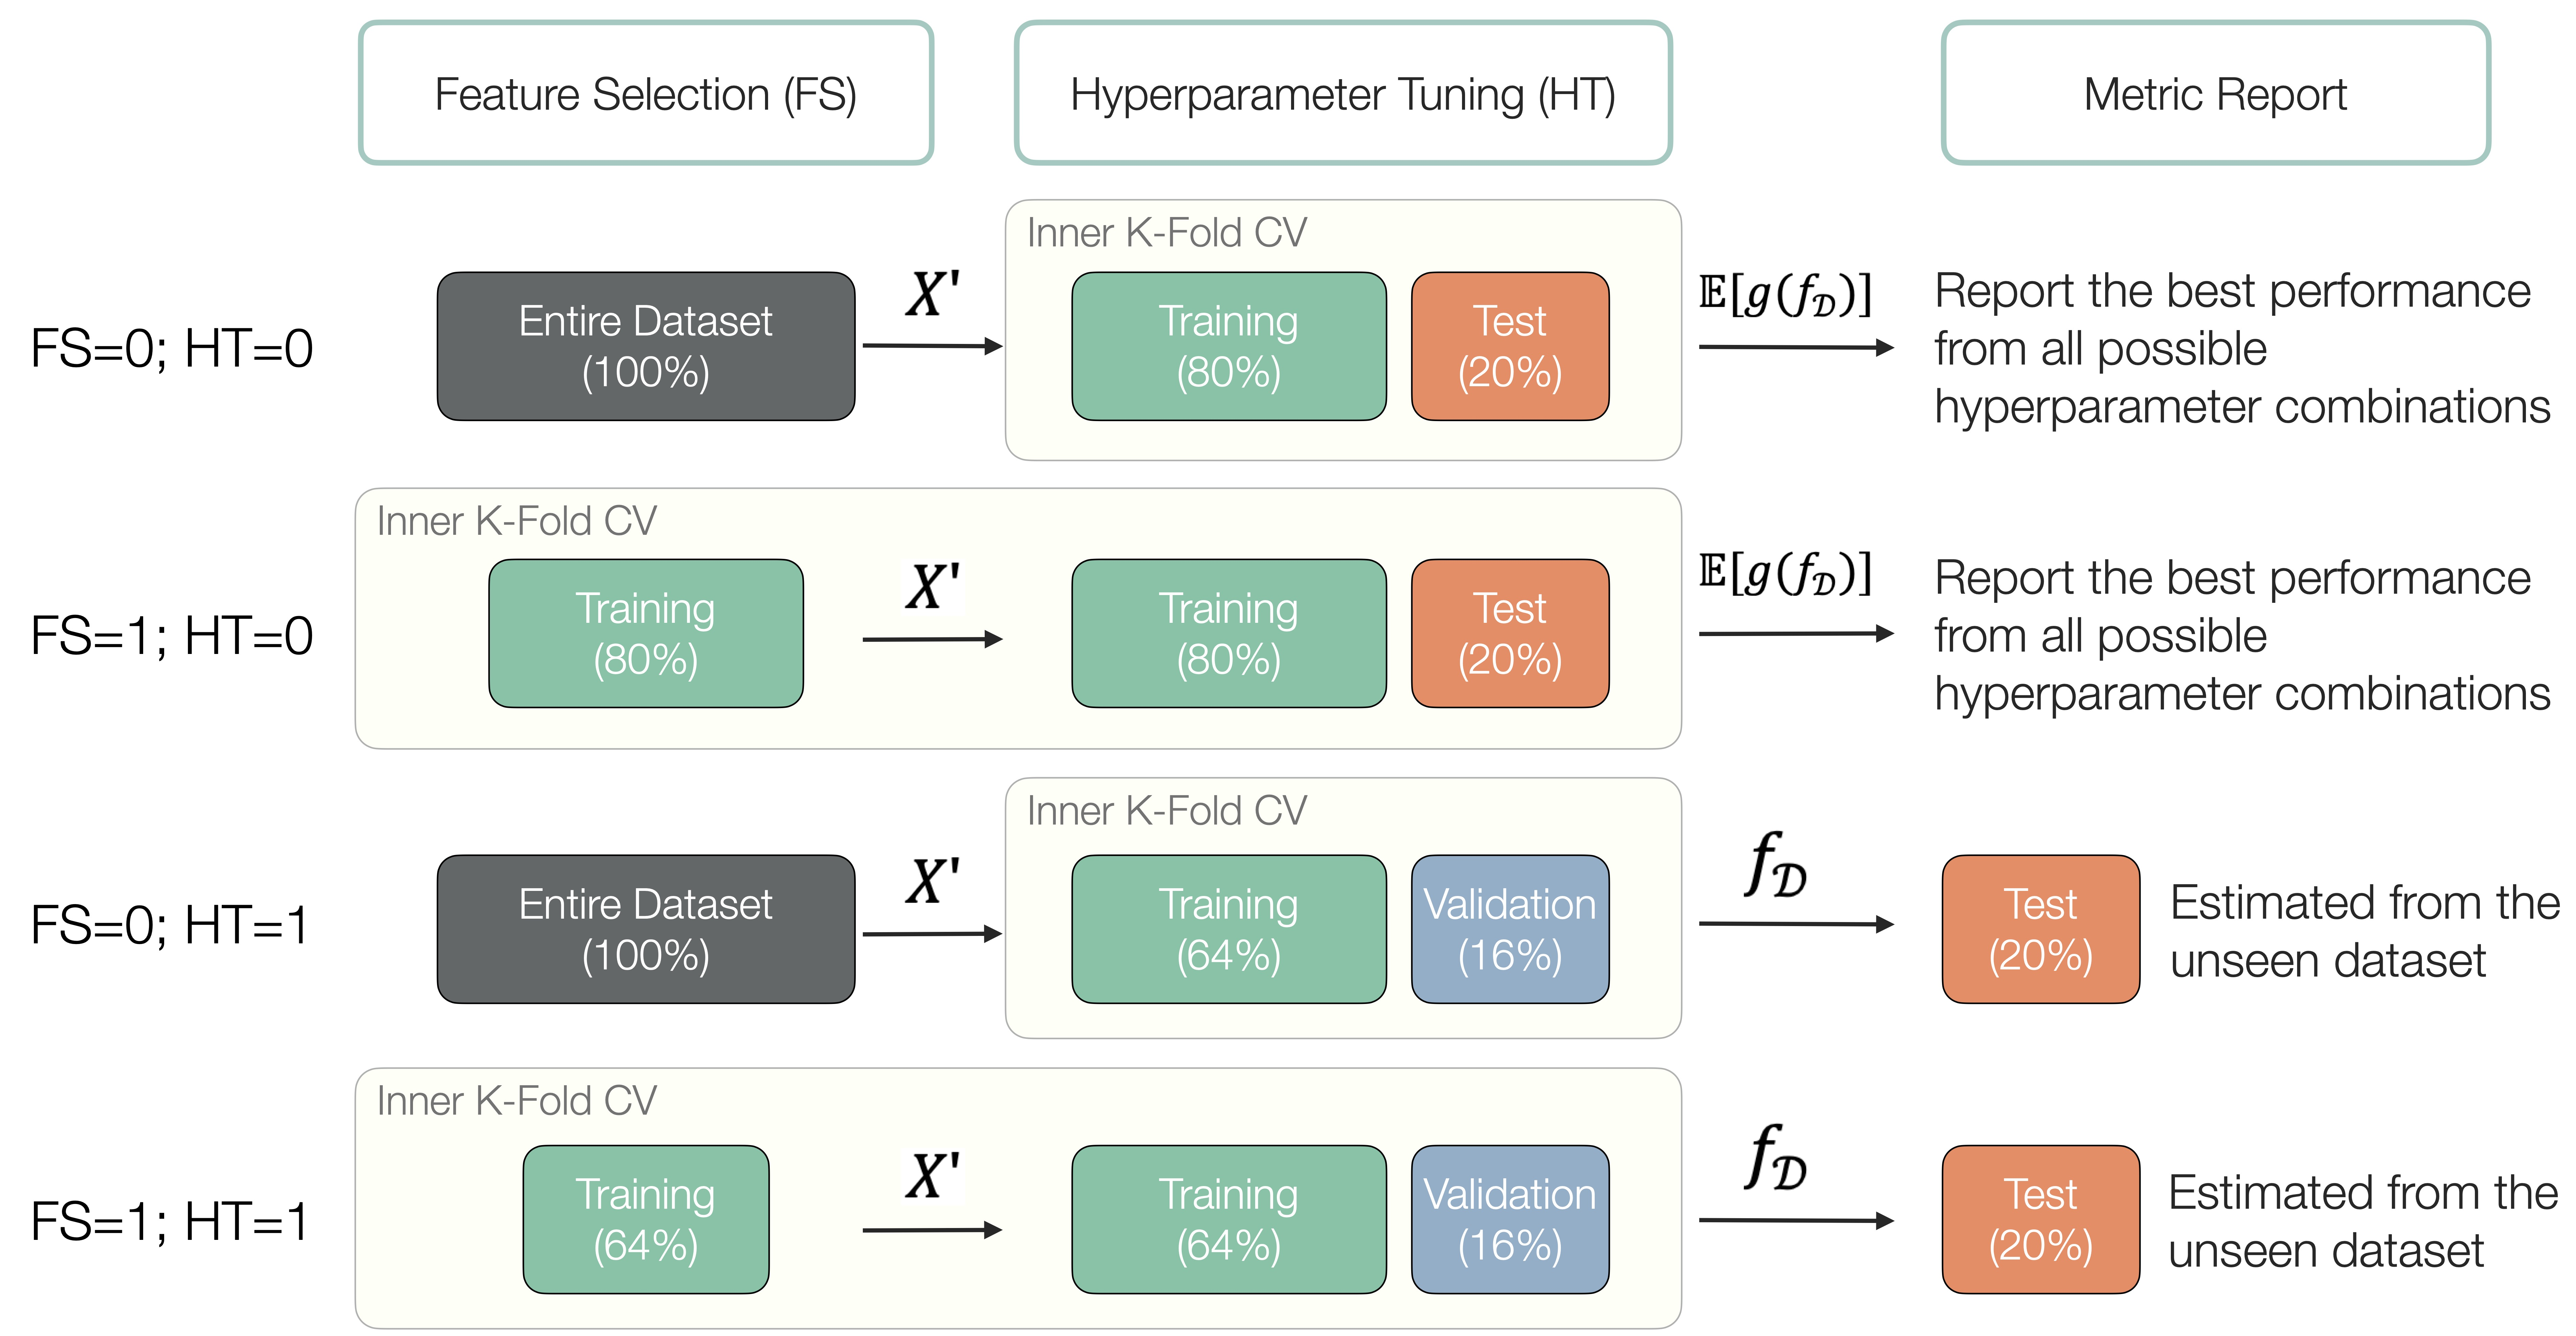
\includegraphics[width=1\textwidth]{fig_s2_schemes.jpg}
    \caption{Workflow diagram illustrating four cross-validation strategies of feature selection (FS) and hyperparameter tuning (HT), where 0 denotes incorrect implementation and 1 indicates correct practice. $X'$ is the selected feature subset, $\mathbb{E}[\hat{g}(f_\mathcal{D})]$ is the expected generalization performance, $f_\mathcal{D}$ is the model trained on the training set without being revealed to the test set.}
    \label{fig:s2_schemes}
\end{figure}

This study introduces notations FS for feature selection and HT for hyperparameter tuning, assigning a binary indicator (0 or 1) to denote incorrect (0) or correct (1) implementation of model selection. This yields four possible combinations of model selection strategies: “FS=0; HT=0”, “FS=0; HT=1”, “FS=1; HT=0”, “FS=1; HT=1” (Figure 7). When FS=0, feature selection precedes cross-validation splitting. If FS=1, feature selection occurs within each fold of the training set during cross-validation. With hyperparameter tuning, a correct implementation (HT=1) involves splitting the dataset into training (64\%), validation (16\%), and test (20\%) sets. The model is trained and tuned using the training and validation sets, respectively, while the test set is reserved for a single evaluation of model performance. Conversely, with HT=0, only training (80\%) and test (20\%) sets are used, risking validation bias as the test set informs both training and performance reporting. A 5-fold cross-validation approach was deployed for all strategies.
Validation bias is measured as the discrepancy between the model selection-influenced performance estimate and the expected generalization performance (r=0), using the Pearson correlation coefficient between predicted and observed values. Over 1000 sampling iterations, the study assesses the distribution of validation bias. A t-test will determine whether the validation bias significantly deviates from zero.

\subsection{Study 3: Block Effects in Cross-Validation}


\section{Results and Discussion}

\subsection{Study 1: The Impact of Estimator Choice and Sample Size on Model Evaluation Reliability}

The simulation results, depicted in box plots (Figure ~\ref{fig:s1_bias} and ~\ref{fig:s1_var}), explored the evaluation bias and variance distribution. Figure ~\ref{fig:s1_bias} examines the bias alterations across various estimators and sample sizes. Independent of the estimator and metric, the bias diminishes with increasing sample sizes. The in-sample estimator consistently overestimates across all metrics and sample sizes, underscoring the necessity of CV for unbiased performance evaluation. In CV estimators, although LOOCV is traditionally viewed as unbiased, it shows underestimation in model performance, especially when the metric is correlation coefficient (r). Comparatively, 2-, 5-, and 10-fold CV provide a more unbiased estimation than LOOCV for all sample sizes. However, for metrics like $R^2$ or RMSE, LOOCV emerges as the least biased estimator. While K-fold CV exhibits higher bias than LOOCV, this difference dwindles when the sample size exceeds 500. Notably, 10-fold CV, contrary to expectations, demonstrates higher bias than 5-fold CV for small sample sizes (50 and 100) in the $R^2$ metric, though this disparity also becomes insignificant at larger sample sizes.

\begin{figure}[h]
    \centering
    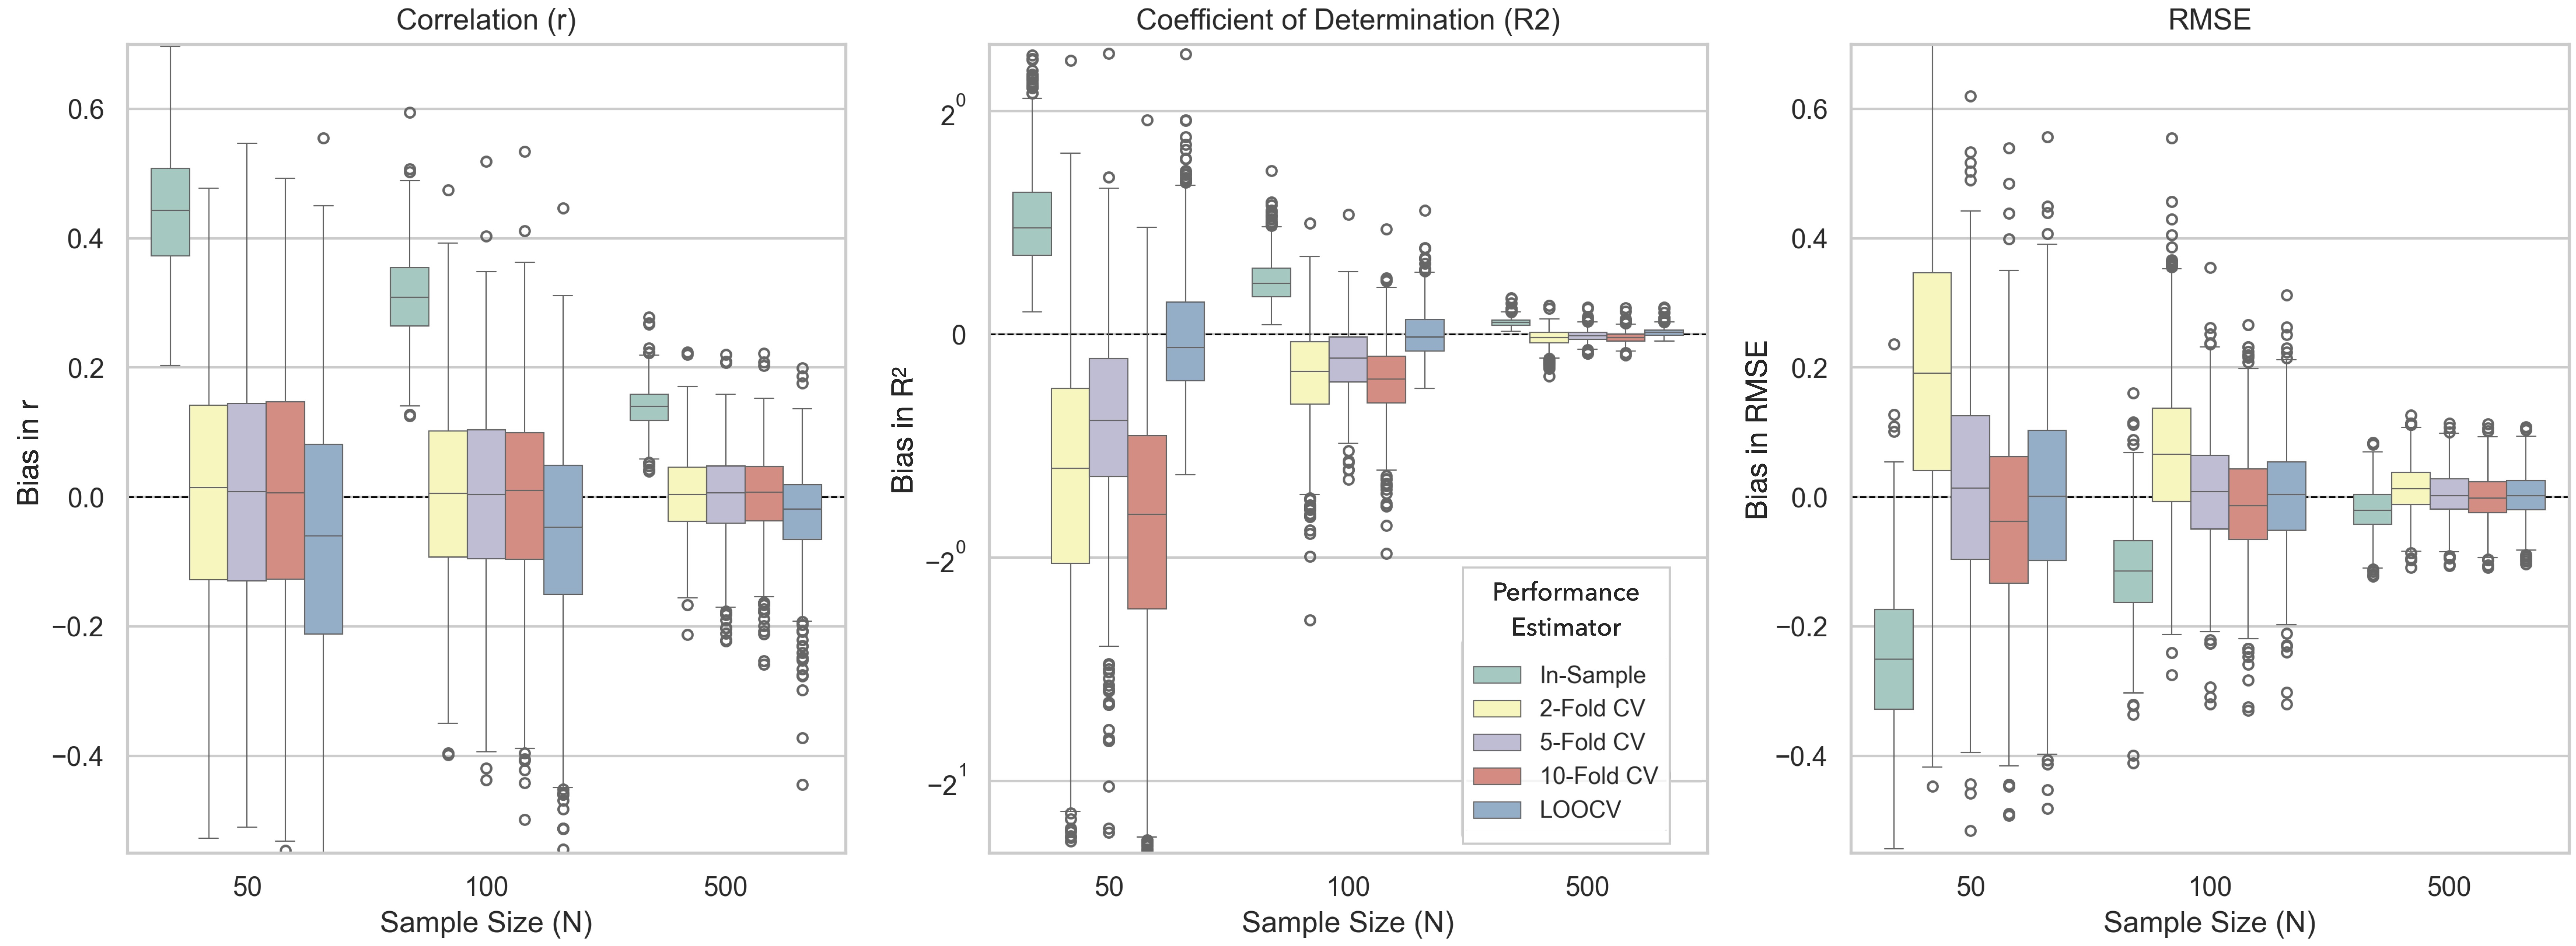
\includegraphics[width=1\textwidth]{fig_1_bias.jpg}
    \caption{Simulation results of evaluation bias from 1000 sampling iterations. Multiple performance estimators across different sample sizes were color-coded. Three metrics: $r$, $R^2$, and RMSE, were displayed in the column facets.}
    \label{fig:s1_bias}
\end{figure}

Considering LOOCV’s singular data point testing, its evaluation variance is pertinent only for RMSE, which permits single data point evaluations. Figure ~\ref{fig:s1_var} illustrates the bias and variance in RMSE across different performance estimators as a function of sample size N. Both bias and variance in RMSE decrease as sample size increases, aligning with the hypothesis. LOOCV provides the least biased estimation, while 2-fold CV exhibits the highest bias without significant reduction at larger sample sizes. However, biases across all estimators converge at a sample size of 500. In terms of evaluation variance, LOOCV consistently shows higher values than other estimators for all sample sizes. Additionally, a lower number of folds K correlates with reduced variance, which is also in line with the hypothesized trend.

\begin{figure}[h]
    \centering
    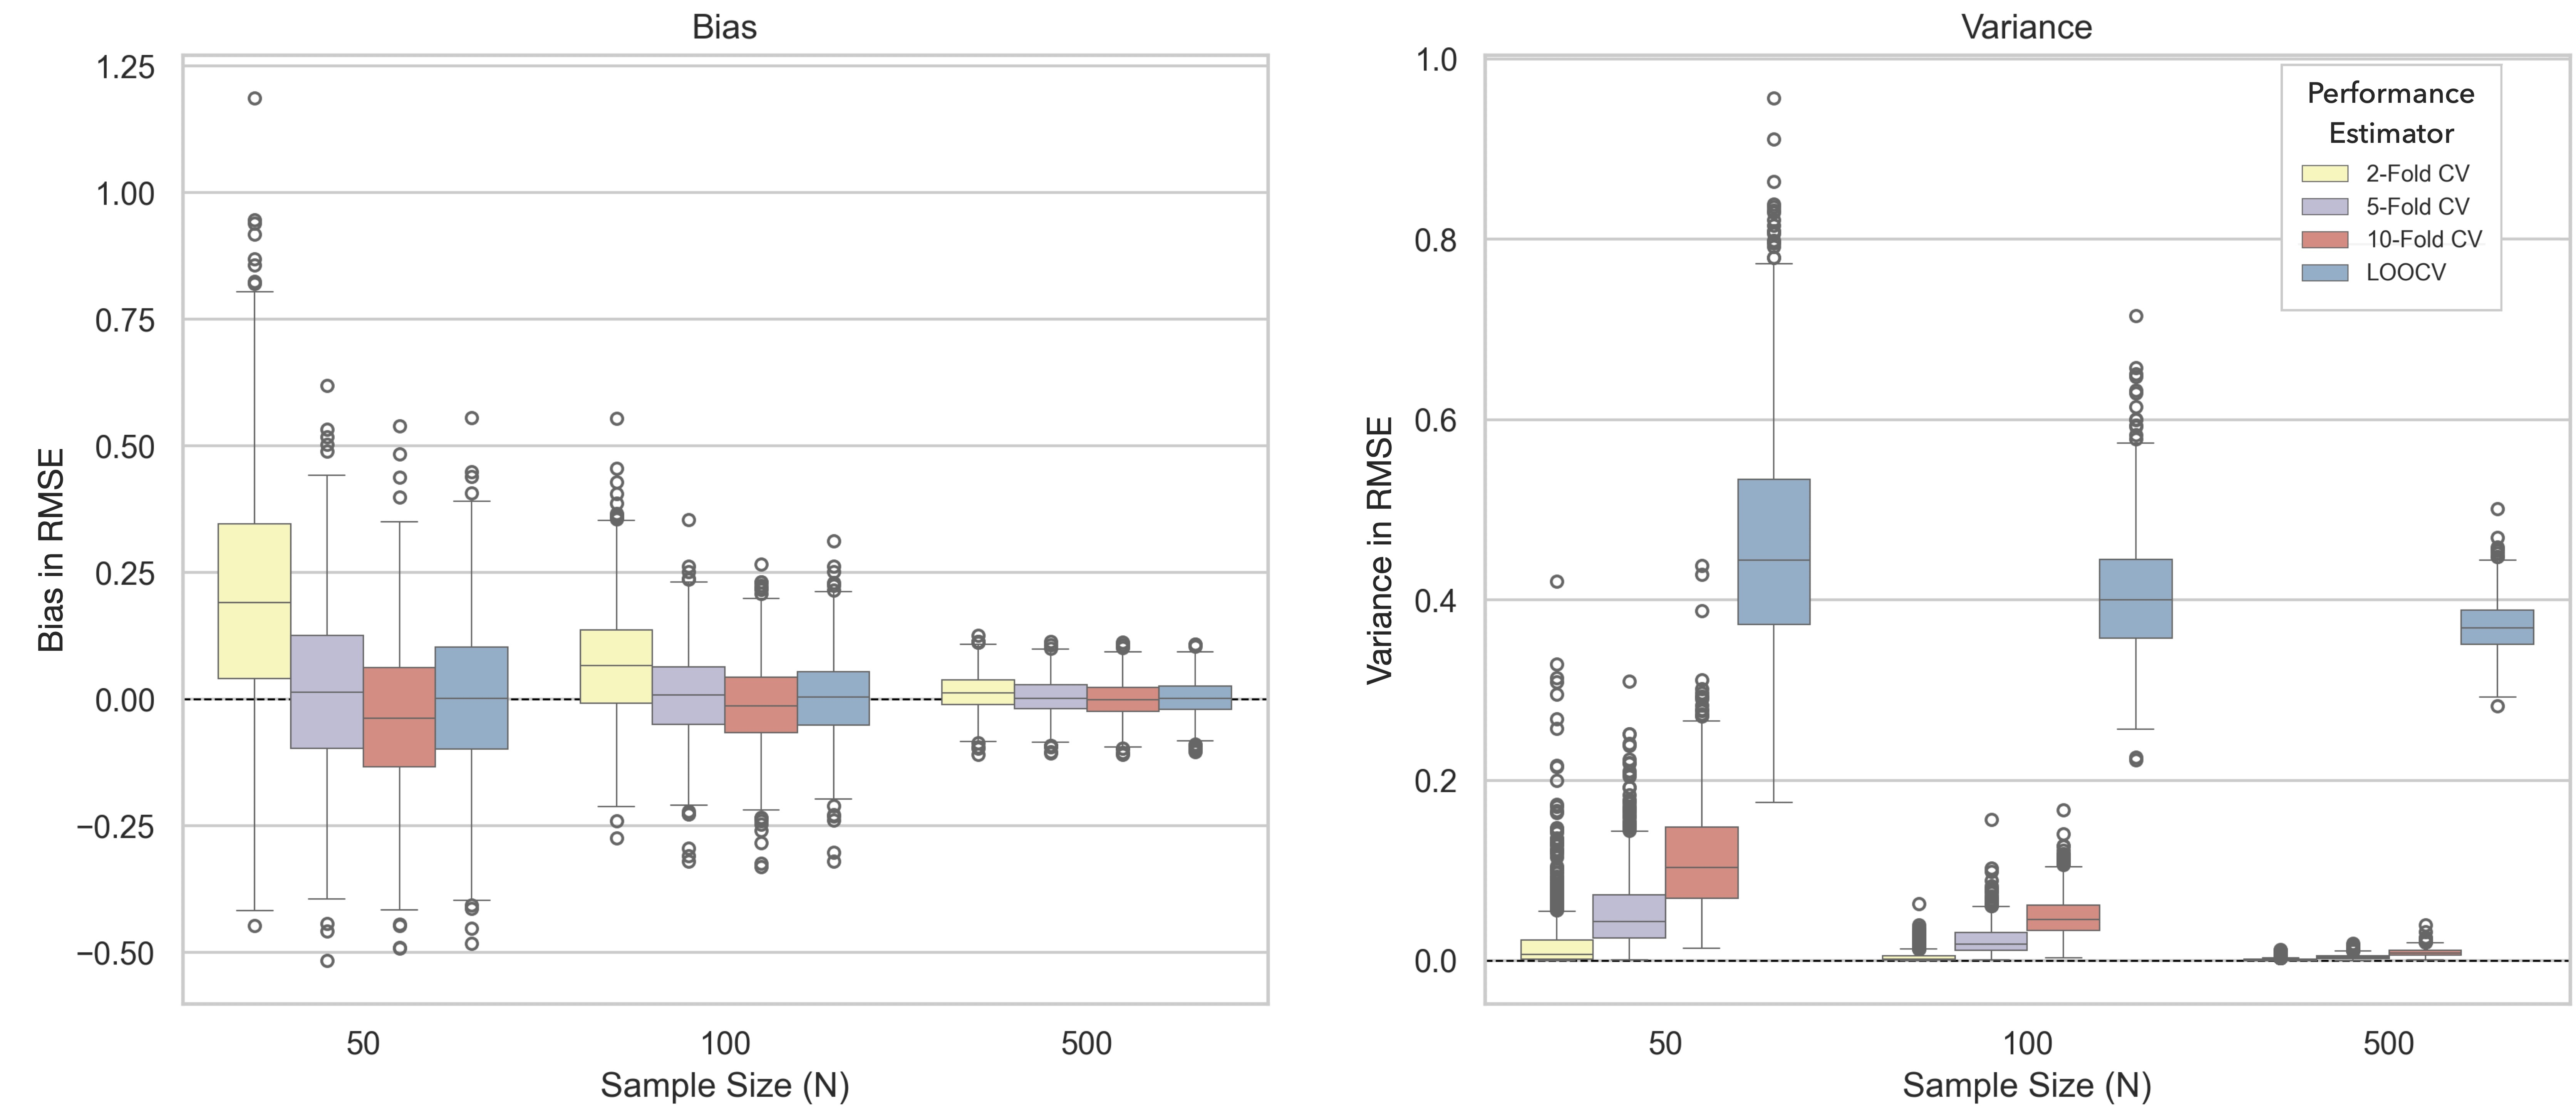
\includegraphics[width=1\textwidth]{fig_1_var.jpg}
    \caption{Simulation results of evaluation bias and variance from 1000 sampling iterations. Multiple performance estimators across different sample sizes were color-coded. Only RMSE was displayed. Bias and variance were listed in the left and right facets, respectively.}
    \label{fig:s1_var}
\end{figure}

In conclusion, when conducting model evaluation, it is crucial to consider the estimator and sample size, as they significantly influence evaluation reliability which can be decomposed into bias and variance. Larger sample sizes generally lead to reduced bias and variance, enhancing the reliability of the evaluation process. For unbiased performance estimation, CV methods, such as K-fold CV and LOOCV, are preferable to in-sample estimation. LOOCV often provides less biased estimations for certain metrics but can exhibit higher variance. It is also noteworthy that the number of folds in K-fold CV can affect bias and variance; thus, experimenting with different numbers of folds, especially in smaller sample sizes, can be beneficial. Ultimately, the selection of appropriate evaluation techniques should be tailored to the specific context of the dataset and the objectives of the modeling exercise, ensuring a robust and reliable assessment of model performance.

\subsection{Study 2: Misuse of Model Selection Can Lead to Over-Optimistic Performance Estimates}

The evaluation bias was visualized using box plots (Figure ~\ref{fig:s2_results}), with the feature selection factor (FS) on the x-axis and hyperparameter tuning (HT) distinguished by color — green for incorrect and yellow for correct implementation. The y-axis represents the evaluation bias as measured by the correlation coefficient. The results indicate a clear overestimation of model performance when feature selection is applied to the entire dataset, regardless of hyperparameter tuning. The median biases were 0.797 for “FS=0; HT=0” and 0.761 for “FS=0; HT=1”. Moreover, inappropriate evaluation in hyperparameter tuning resulted in a significant bias (p-value < 0.001) with a median of 0.113 for “FS=1; HT=0”. The only scenario without bias significantly occurred when both feature selection and hyperparameter tuning were correctly incorporated within the cross-validation process “FS=1; HT=1”, yielding a median bias of -0.008. These findings align with the initial hypothesis and the prevailing literature, reinforcing that model selection must be integrated into the cross-validation workflow to prevent an overestimation of model performance.

\begin{figure}[h]
    \centering
    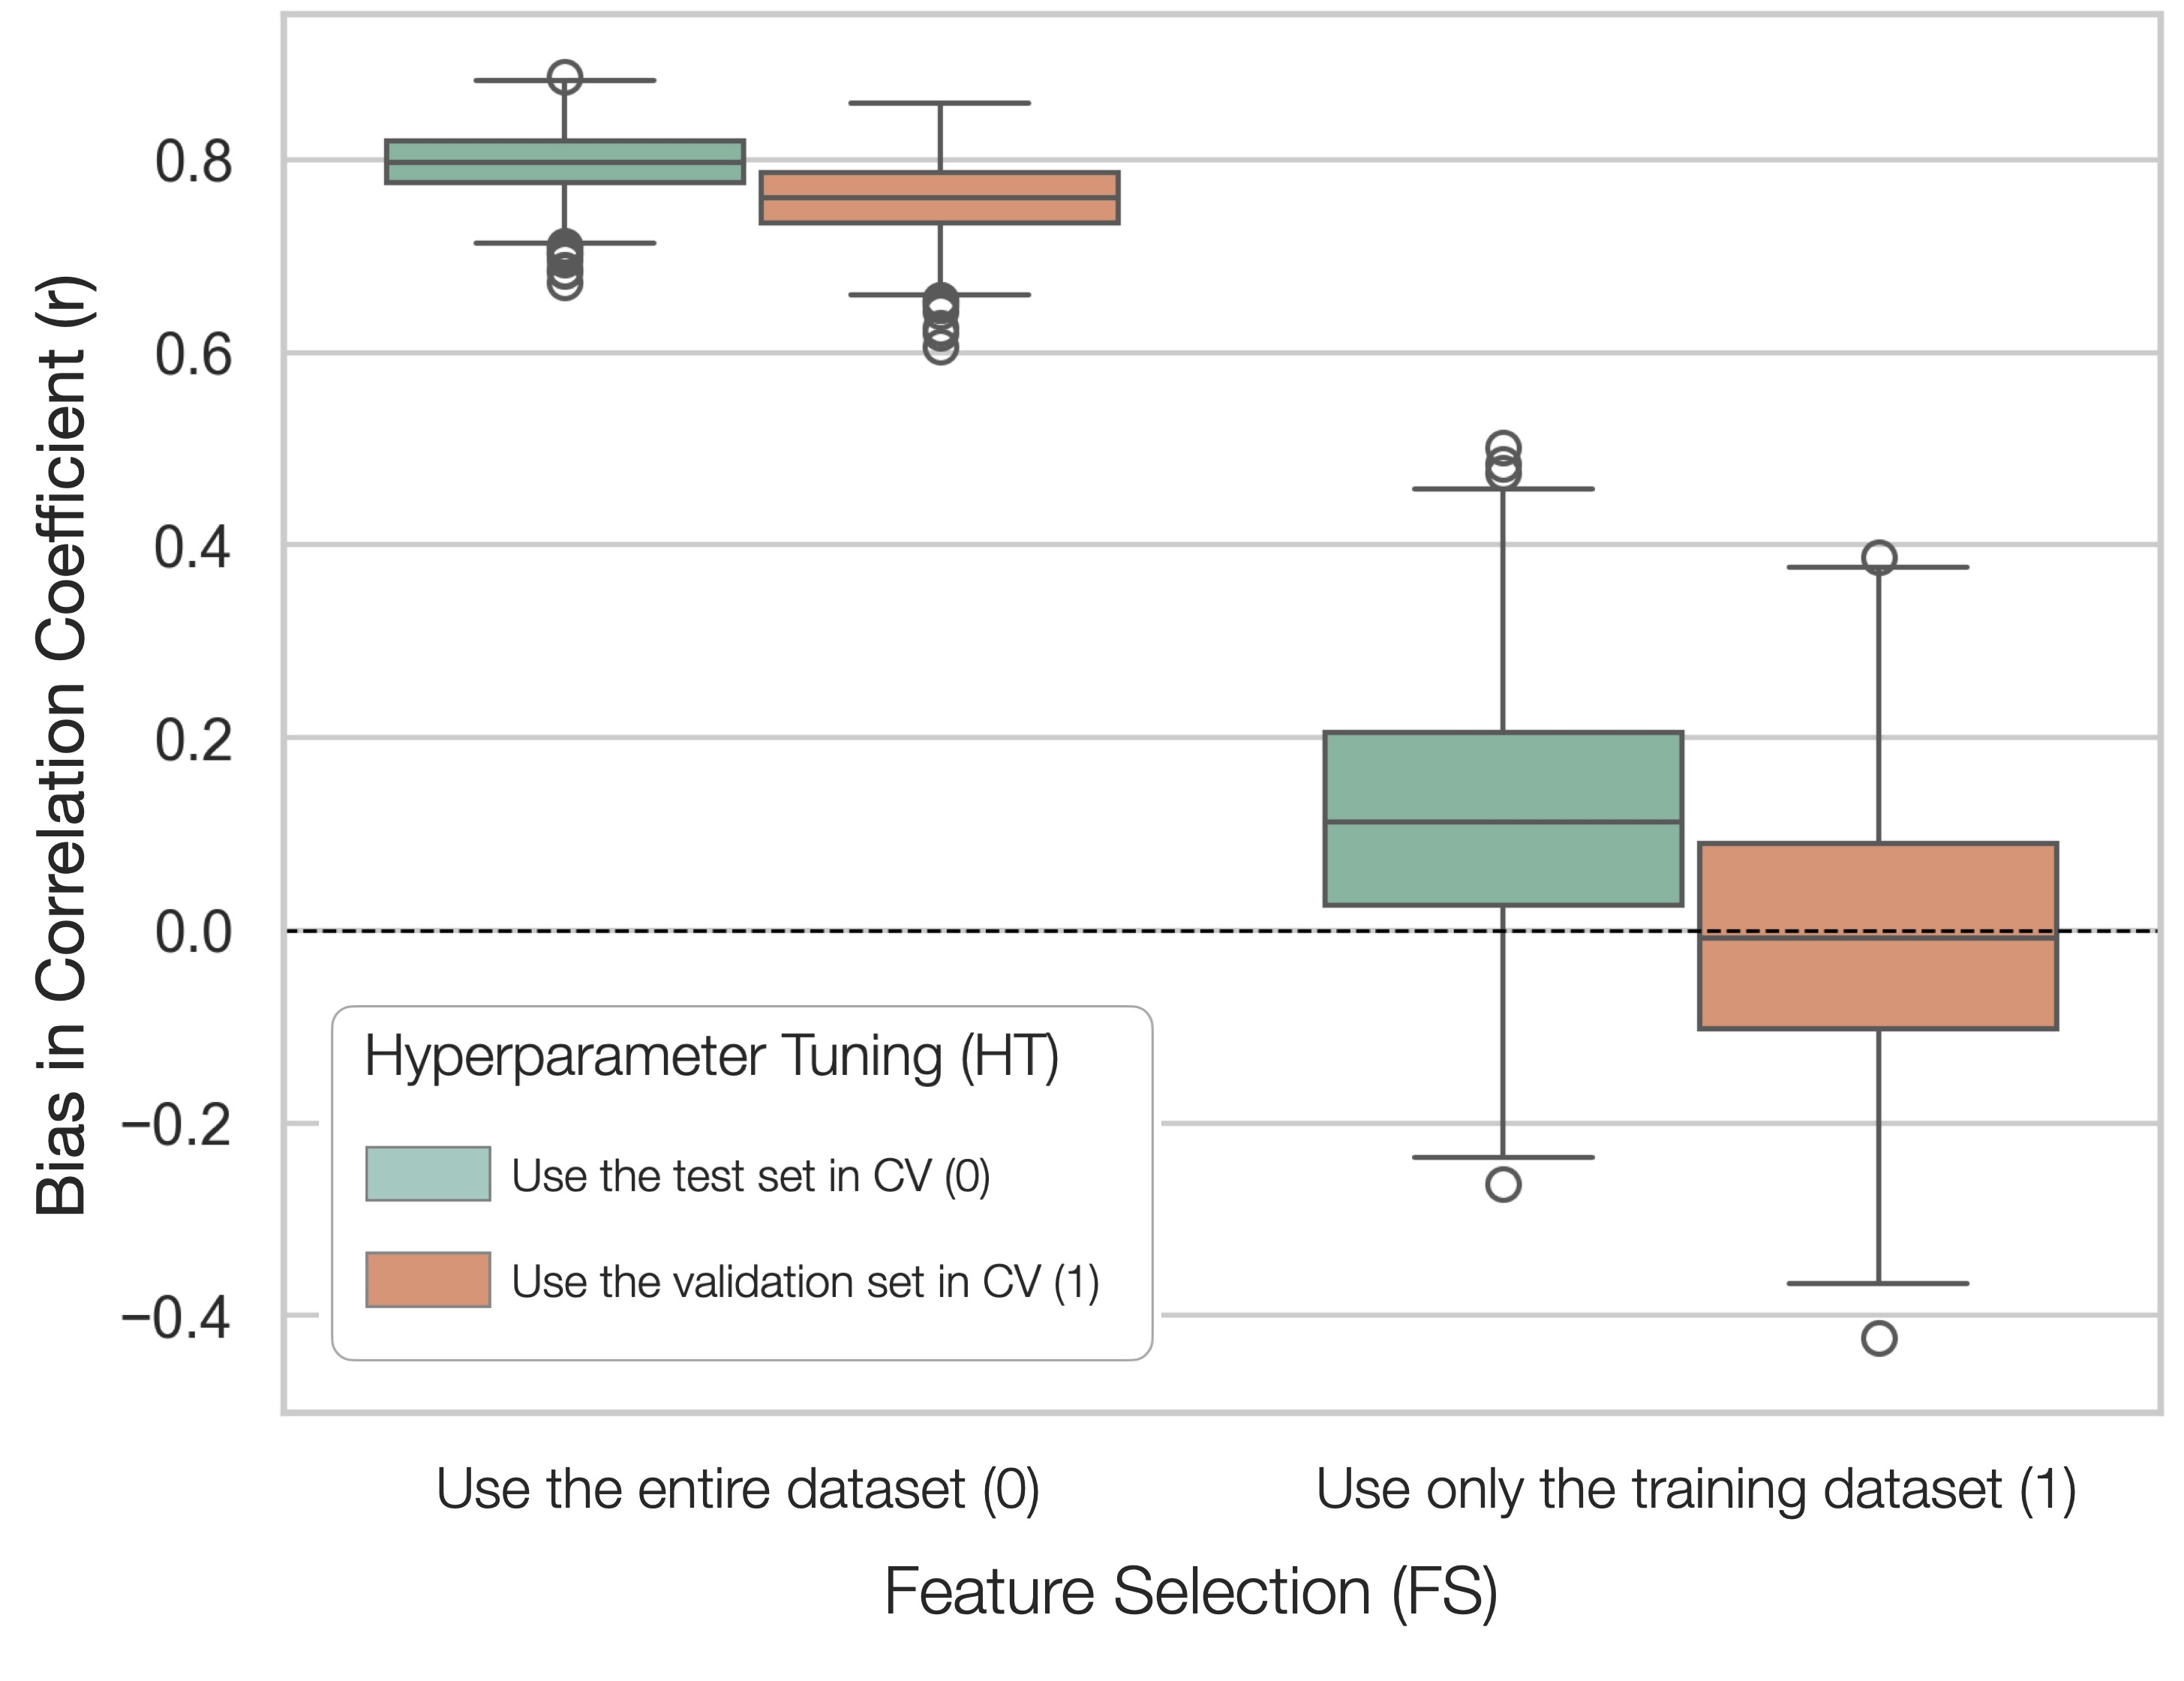
\includegraphics[width=.7\textwidth]{fig_s2_results.jpg}
    \caption{The evaluation bias of the four model selection strategies.}
    \label{fig:s2_results}
\end{figure}

The simulation results robustly confirm the hypothesis that improper implementation of model selection inflates performance estimates. Specifically, the evaluation bias is markedly high when feature selection precedes data splitting, with or without correct hyperparameter tuning. Although integrating feature selection within cross-validation folds mitigates this bias, incorrect hyperparameter tuning still significantly skews performance metrics. Notably, this overestimation from the hyperparameter tuning is even more pronounced in complex models, such as neural network architectures that often entail over a million parameters. These findings underscore the necessity of meticulous cross-validation practices, particularly for feature selection and hyperparameter tuning, to ensure accurate performance estimations and generalizability in predictive modeling.

\subsection{Study 3: Overlooking Experimental Block Effects Can Lead to Biased Model Performance Estimates}

In this simulation, an ANOVA table (Table ~\ref{tab:anova}), calculated from a single iteration for illustrative purposes, demonstrates that the simulated data exhibits block variation significantly greater than the residual variance. The result (Figure ~\ref{fig:s3_results}) shows that regardless of the amplitude of block effects in this simulation study, the Block CV strategy consistently yields a mean performance estimate close to zero, while the Random CV strategy consistently and significantly overestimates the model performance (p-value < 0.001). This finding supports the hypothesis that Random CV tends to overestimate model performance when block variation predominates over residual variation.

\begin{table}
    \caption{ANOVA results for a single iteration of the simulated data with b = 0.5. SS: sum of squares; DF: degree of freedom; MS: mean square; F: F-statistic}
    \centering
    \begin{tabular}{lccccc}
        \toprule
        Source & SS & DF & MS & F & p-value \\
        \midrule
        Between & 60.971 & 4 & 15.243 & 20.580 & <0.001 \\
        Within & 70.363 & 95 & 0.741 & &  \\
        \cmidrule(r){1-3}
        Total & 131.35 & 99 & & & \\
        \bottomrule
    \end{tabular}
    \label{tab:anova}
\end{table}

In conclusion, block CV proves to be a vital tool in assessing the generalizability and accuracy of a predictive model, especially in contexts where block effects, such as herd variations, play a significant role in both the predicting features and response variable. The random CV strategy, which randomly assigns samples to folds without considering block effects, tends to overestimate model performance. This study recommends that block CV be used as a benchmark in model validation, especially when block effects are present

\begin{figure}[h]
    \centering
    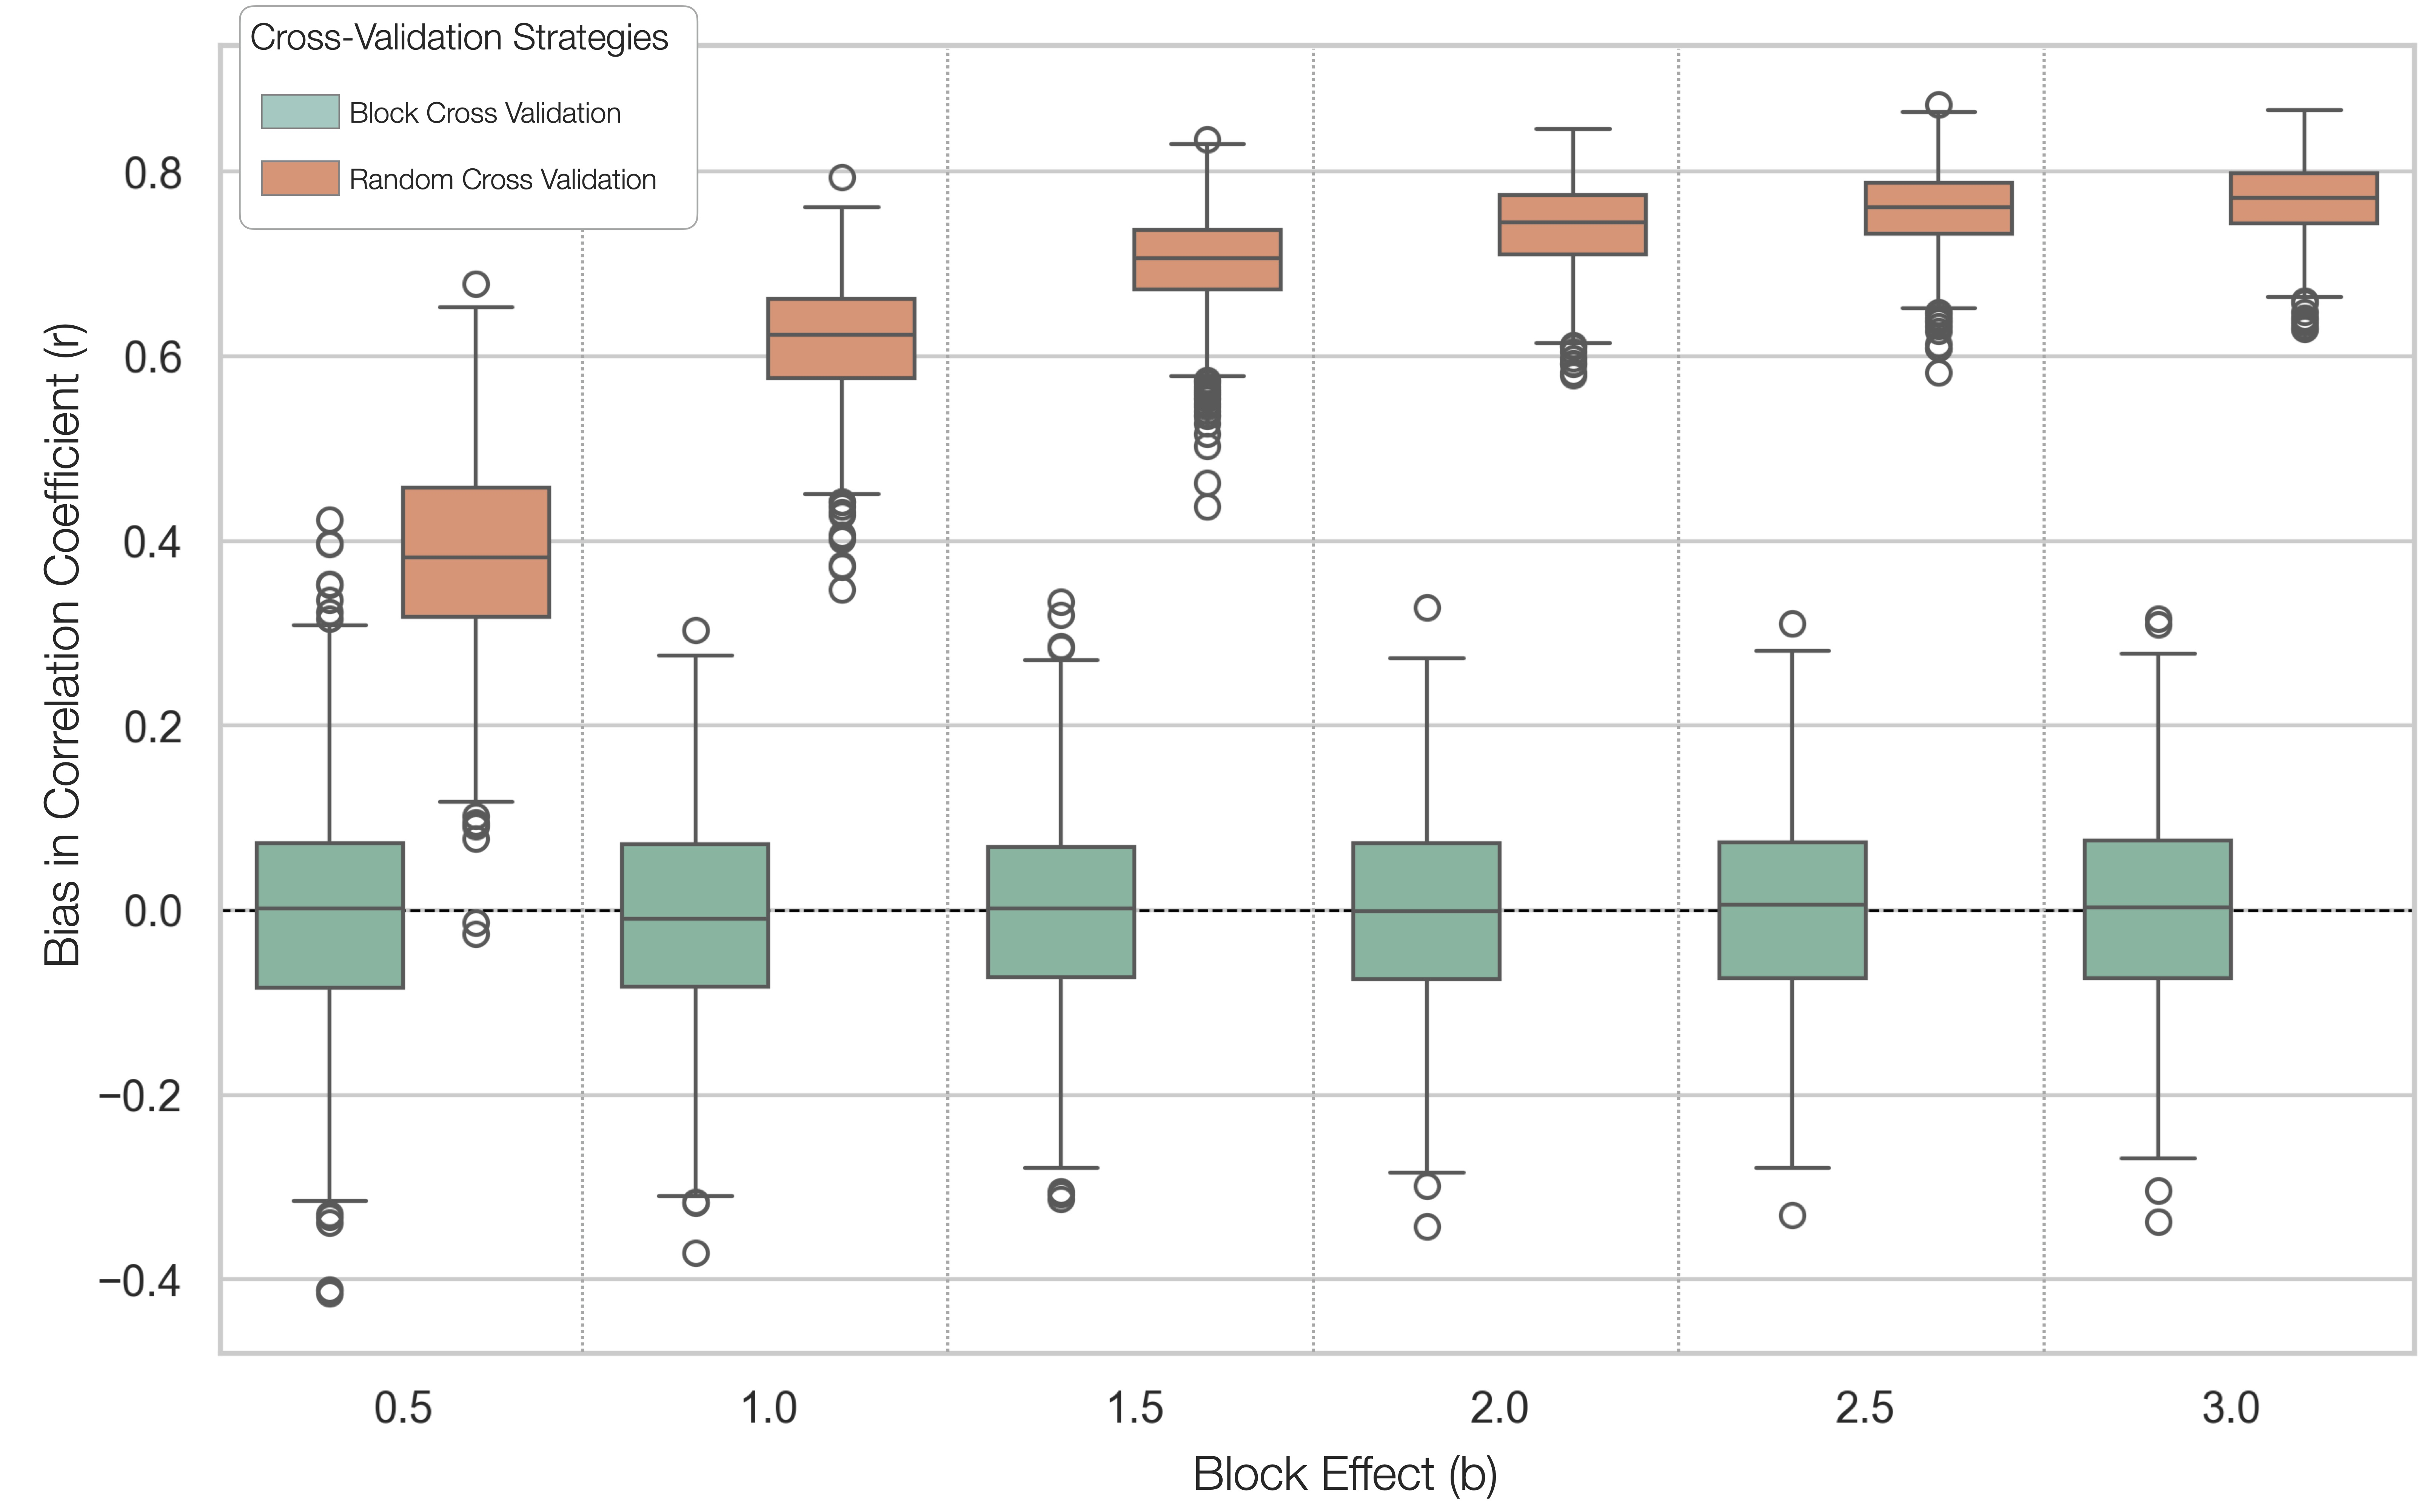
\includegraphics[width=1\textwidth]{fig_s3_results.jpg}
    \caption{Bias in model performance estimation by Block CV and Random CV across 1000 iterations. The dashed line represents the null hypothesis that the mean performance estimate is zero.}
    \label{fig:s3_results}
\end{figure}

\subsection{Study 4: Different Regression Metrics Illustrate Different Aspects of Model Performance}

\begin{figure}[h]
    \centering
    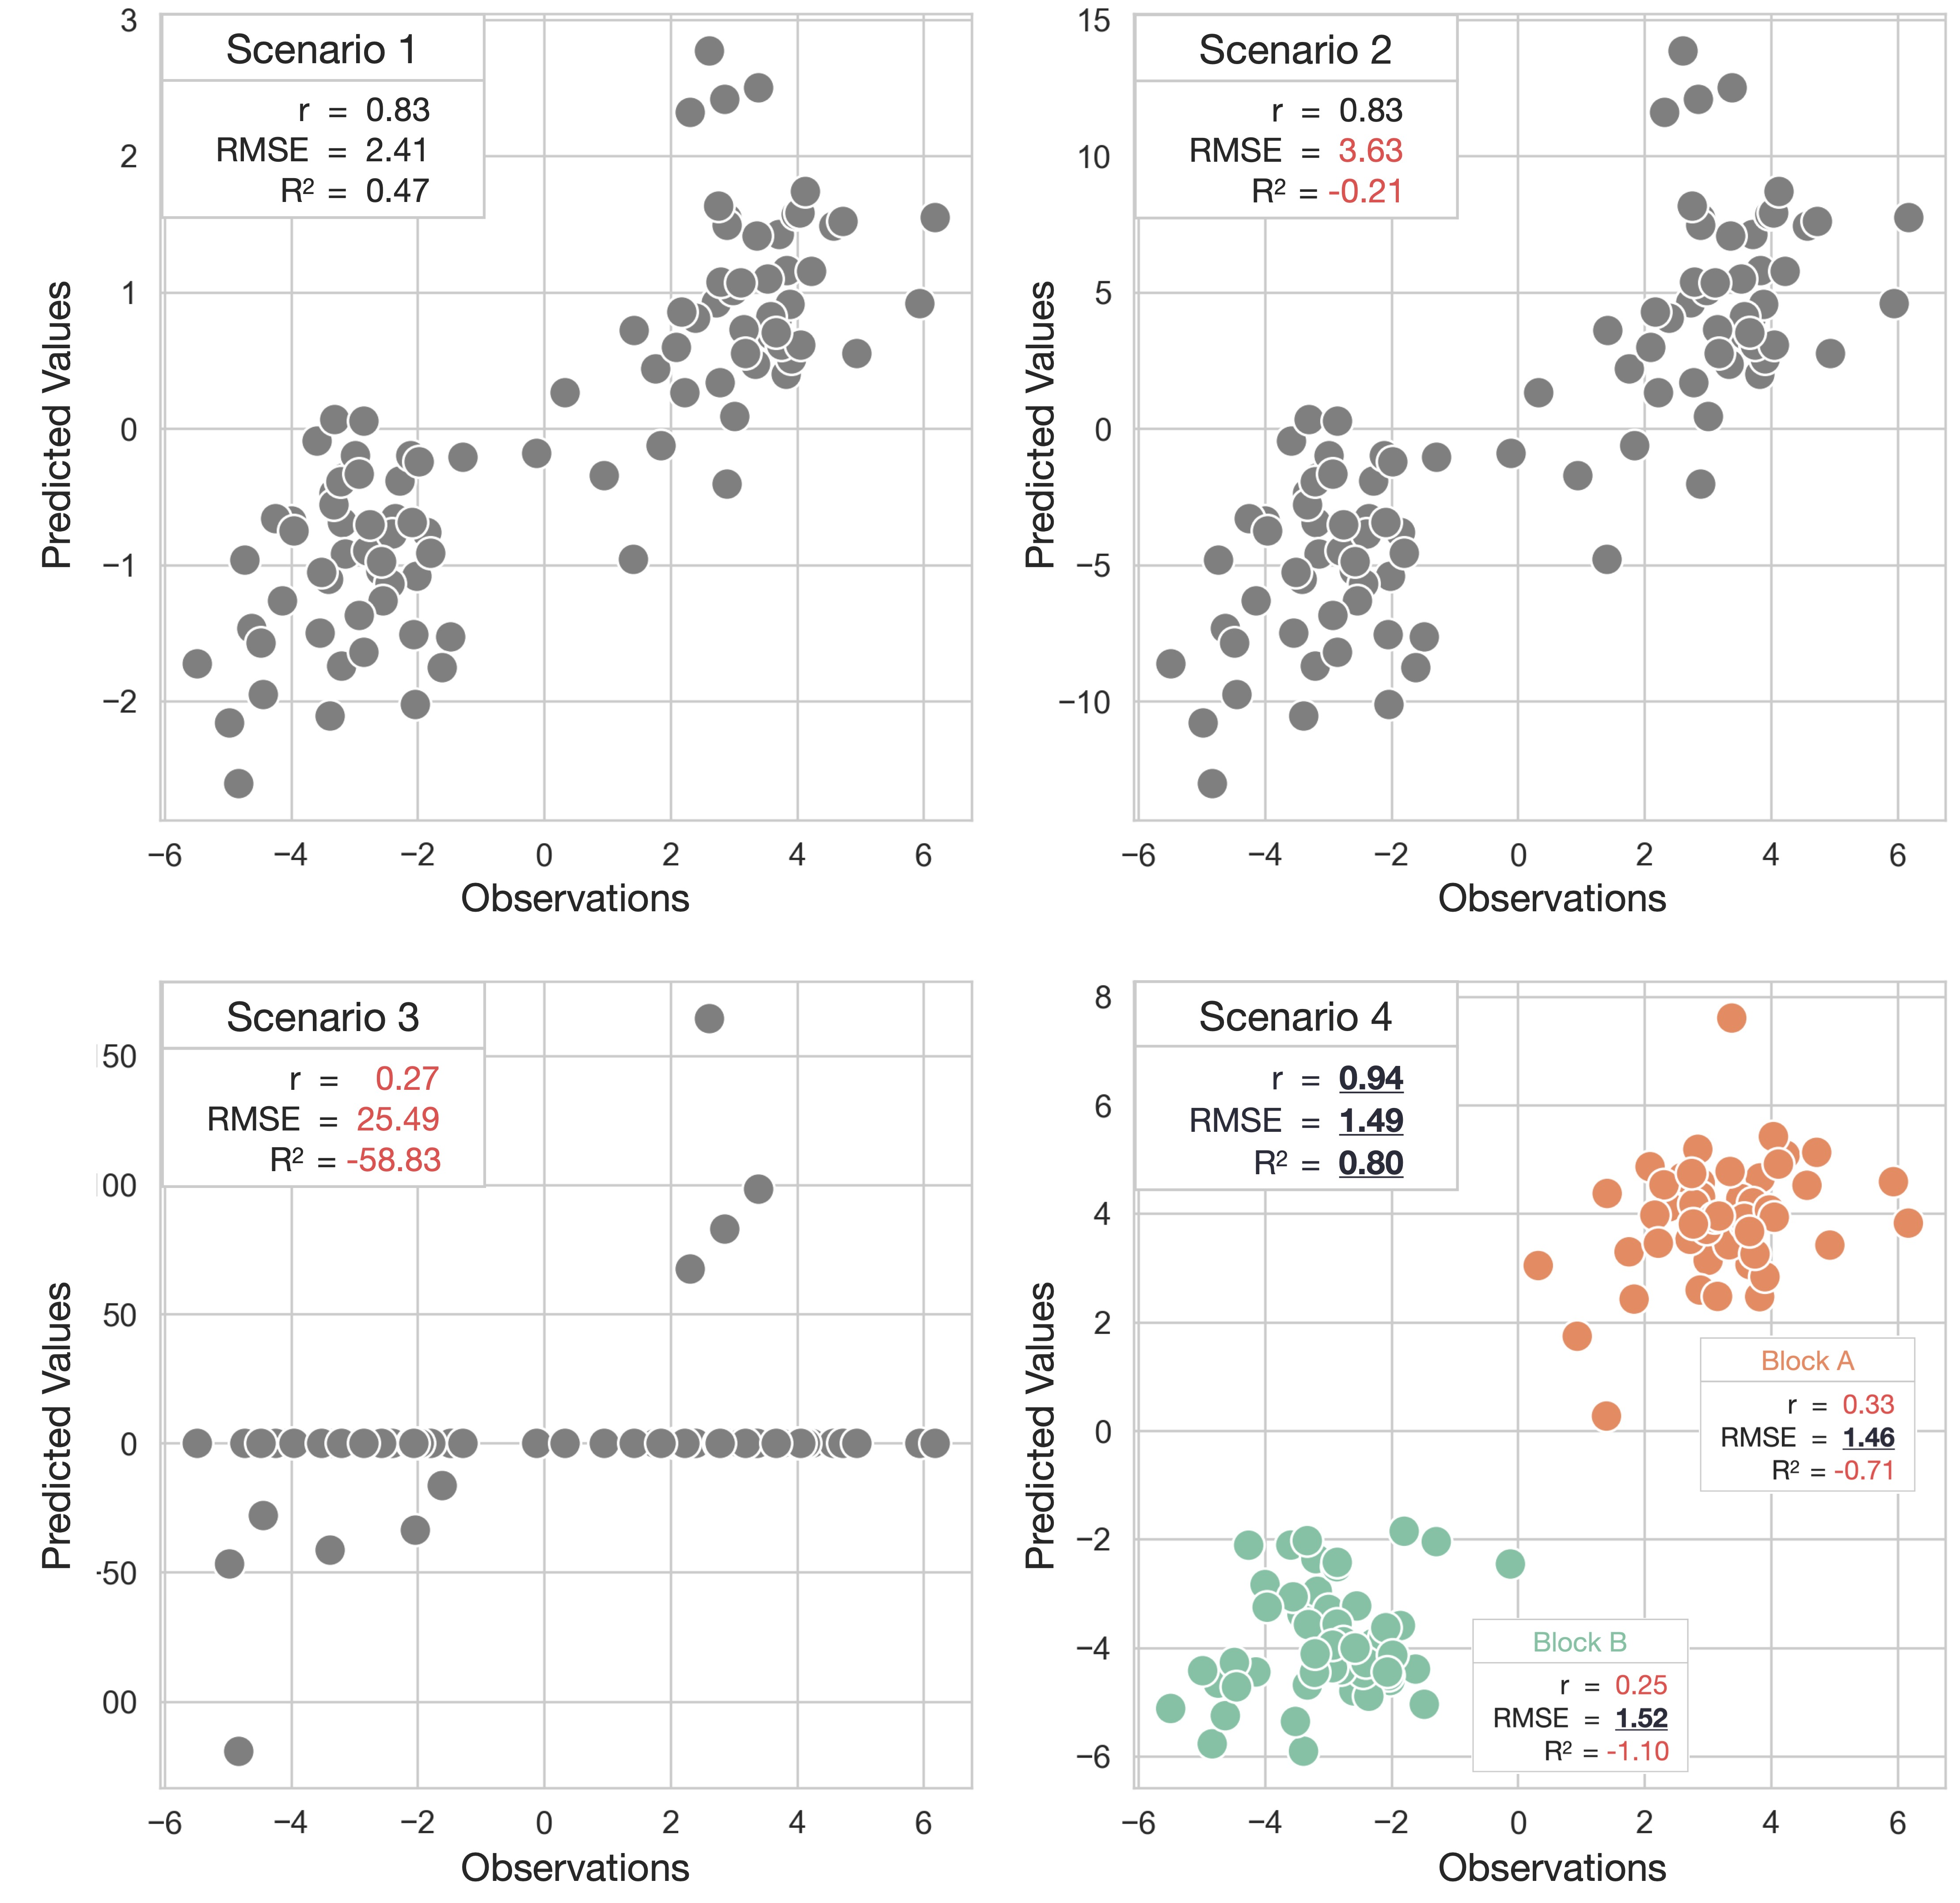
\includegraphics[width=.8\textwidth]{fig_s4_reg.jpg}
    \caption{Scatter plots display the same observations against four different prediction scenarios in the given hypothetical example. Scenario 1 serves as a baseline for the metrics, with any metric better than the baseline highlighted in bold and underscored, and any worse metric colored in red.}
    \label{fig:s4_reg}
\end{figure}

The simulated hypothetical example in Figure ~\ref{fig:s4_reg} illustrates the performance of four different prediction scenarios. When the goal is to rank observations of interest rather than predict the absolute magnitude of the error, this metric is appropriate. The property of this metric was demonstrated in both Scenario 1 and 2, where the coefficient remained consistent despite Scenario 2 having errors five times greater than in Scenario 1. If the absolute error is of interest, this metric should be used in conjunction with other metrics, such as RMSE or $R^2$. It is also worth noting that this metric can provide a value of 0.27 in Scenario 3, where 90\% of the predictions failed to capture the trend and resulted in zero-value predictions. The positive performance of the metric came from the predictions ranking the remaining 10\% of the observations in a fairly accurate order, regardless of the large error magnitude. Moreover, one common pitfall of this metric is that block effects can influence it, leading to an inflated performance estimate if individual variation is of greater interest than inter-block variation. This was demonstrated in Scenario 4, where the overall coefficient r was 0.94, but the metric within each block was only 0.33 and 0.25, respectively. Therefore, it is essential to visually inspect regression results through scatter plots or examine them within individual blocks.
Distinct from the correlation coefficient $r$, RMSE is sensitive to scale, implying that achieving predictions with a variance akin to the observed values takes precedence over maintaining their order or trend. This property is evident in Scenario 2, where the RMSE inflates from 2.41 to 3.63, despite the fact that the predictions in both scenarios rank the observations identically. Another notable characteristic of RMSE is it weighs more on large errors, which is essential when making a large error is costly and should be prioritized for avoidance. In Scenario 3, where certain predictions deviate substantially from the majority, the squaring operation in Equation ~\ref{eq_rmse} accentuates these outliers, culminating in an RMSE value of 25.49. It is also worth mentioning that RMSE is impervious to block effects, which was illustrated in Scenario 4. In this scenario, both the complete set of predictions and the intra-block predictions yield similar RMSE values—1.49, 1.46, and 1.52, respectively. This phenomenon emphasizes again that RMSE is affected solely by the magnitude of the error, which neglects the ability of the model to capture relative trends in intra-block or inter-block predictions.
In Scenario 1, a moderate $R^2$ of 0.47 indicates that the model explains nearly half of the observed variation. With a five times larger variance compared to Scenario 1, Scenario 2 yields a negative $R^2$ of -0.21 despite retaining the same prediction order. Similarly to RMSE, where errors are squared, the presence of outliers leads to a dramatic $R^2$ drop to -58.83, showcasing the sensitivity of $R^2$ to outlier-induced variance. Lastly, in Scenario 4, the value of $R^2$ indicated a strong performance by the model with a score of 0.80. This score is statistically reasonable, as the model explained 80\% of the total variation, which was mainly contributed by block effects. However, when each block was analyzed individually, the $R^2$ values decreased to -0.71 and -1.10, respectively, because the model failed to account for intra-block variation. In summary, while both RMSE and $R^2$ aim to measure prediction errors, $R^2$ offers additional statistical insights that facilitate a more nuanced evaluation of model performance.
All three metrics discussed in this section are effective in examining the performance of regression models. Correlation Coefficient r evaluates the ability of the model to rank the observations. RMSE is a metric that is easy to interpret and is suitable to evaluate the absolute error. The coefficient of determination $R^2$ measures the proportion of variation that the model can explain. Choosing the appropriate metric hinges on the specific goals of model evaluation. For a thorough analysis, employing multiple metrics is advisable to gain a multifaceted view of the model's performance.

\subsection{Study 5: Label-Invariant Metrics Provide Balanced Assessment in Binary Classification}

\begin{figure}[h]
    \centering
    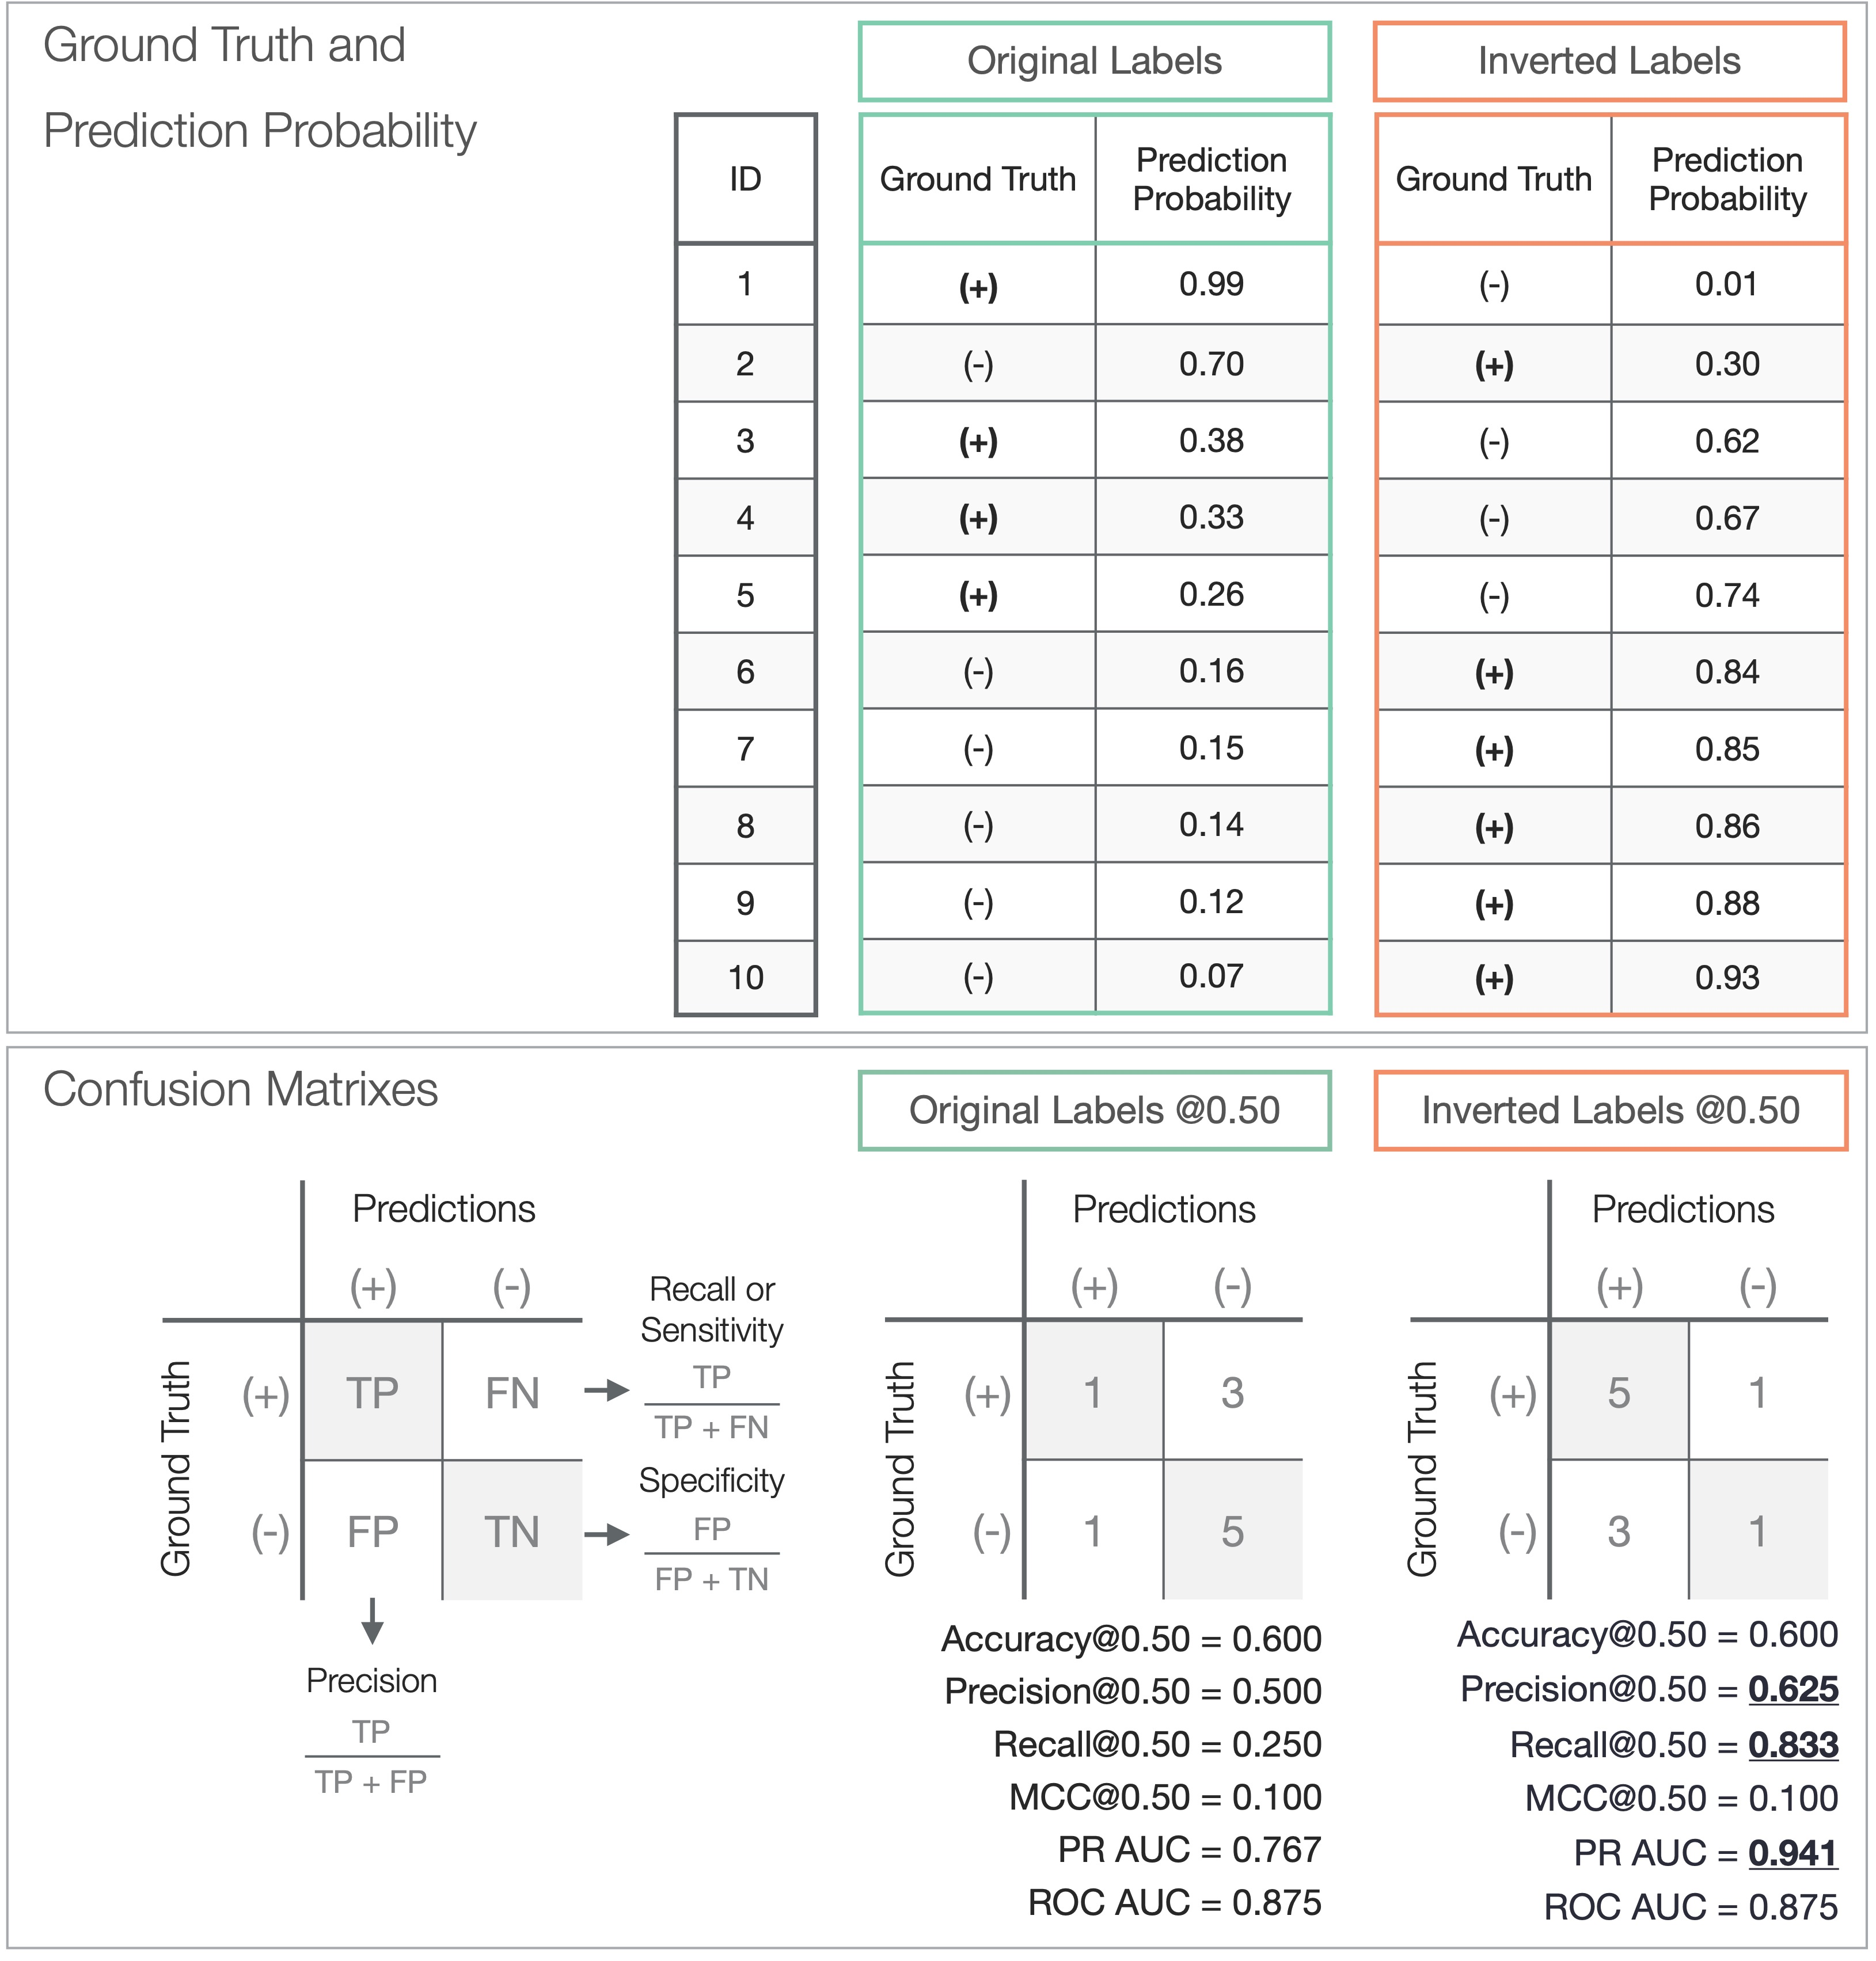
\includegraphics[width=.8\textwidth]{fig_s5_cls.jpg}
    \caption{Simulated hypothetical example of binary classification. TP: true positive; FN: false negative; FP: false positive; TN: true negative; \textbf{Upper}: The ground truth and prediction probability. \textbf{Lower}: The confusion matrix of the prediction at a threshold of 0.5, followed by classification metrics of accuracy, precision, recall, MCC, PR curve AUC, and ROC curve AUC. The performance of the original labels serves as a baseline for comparison. Any better performance metrics from the inverted labels are highlighted in bold and underscored}
    \label{fig:s5_cls}
\end{figure}


Different metrics in binary classification were evaluated in a simulated example (Figure ~\ref{fig:s5_cls}). The original labels were inverted to examine the robustness of the metrics against label choices. The accuracy metric, with a 0.5 threshold in this example, stands at 0.60. This figure might suggest modest efficacy, marginally surpassing random chance, with an accuracy of 0.50. Nonetheless, the same accuracy level could be achieved by classifying every sample as negative in an imbalanced dataset where negatives are predominant. In contrast, precision and recall provide a more nuanced evaluation of model performance by separately assessing the correctness of positive predictions and the ability to detect actual positives. With a threshold of 0.5, the example dataset yields precision and recall values of 0.5 and 0.25, respectively. These metrics deliver more interpretable information that only half of the positive predictions are correct, and just a quarter of the actual positives are detected. This contrasts with an accuracy of 0.6, which may appear misleadingly high due to the abundance of negative samples.
Additionally, it is noted that the chosen confidence threshold significantly impacts precision and recall. While the trade-off between these two metrics is not always linear, it is generally observed that a higher threshold increases precision but decreases recall, and vice versa. A high threshold indicates a conservative approach in predicting positives, reducing false positives, and thus enhancing precision. However, this often leads to missing actual positive cases, lowering recall. Hence, the Precision-Recall (PR) curve is an essential tool for evaluating model performance across various thresholds. Plotted with recall on the x-axis and precision on the y-axis, this curve is derived by computing these metrics at different thresholds (Figure ~\ref{fig:s5_curve}, Left). The Area Under the Curve (AUC) provides a summary measure of the PR curve's overall performance. A model's effectiveness is generally indicated by how close a point on the PR curve is to the top-right corner. For example, at a threshold of 0.25, which is positioned near the top-right of the PR curve, the model demonstrates impressive performance with an accuracy of 0.90, precision of 0.80, and recall at 1.00.

\begin{figure}[h]
    \centering
    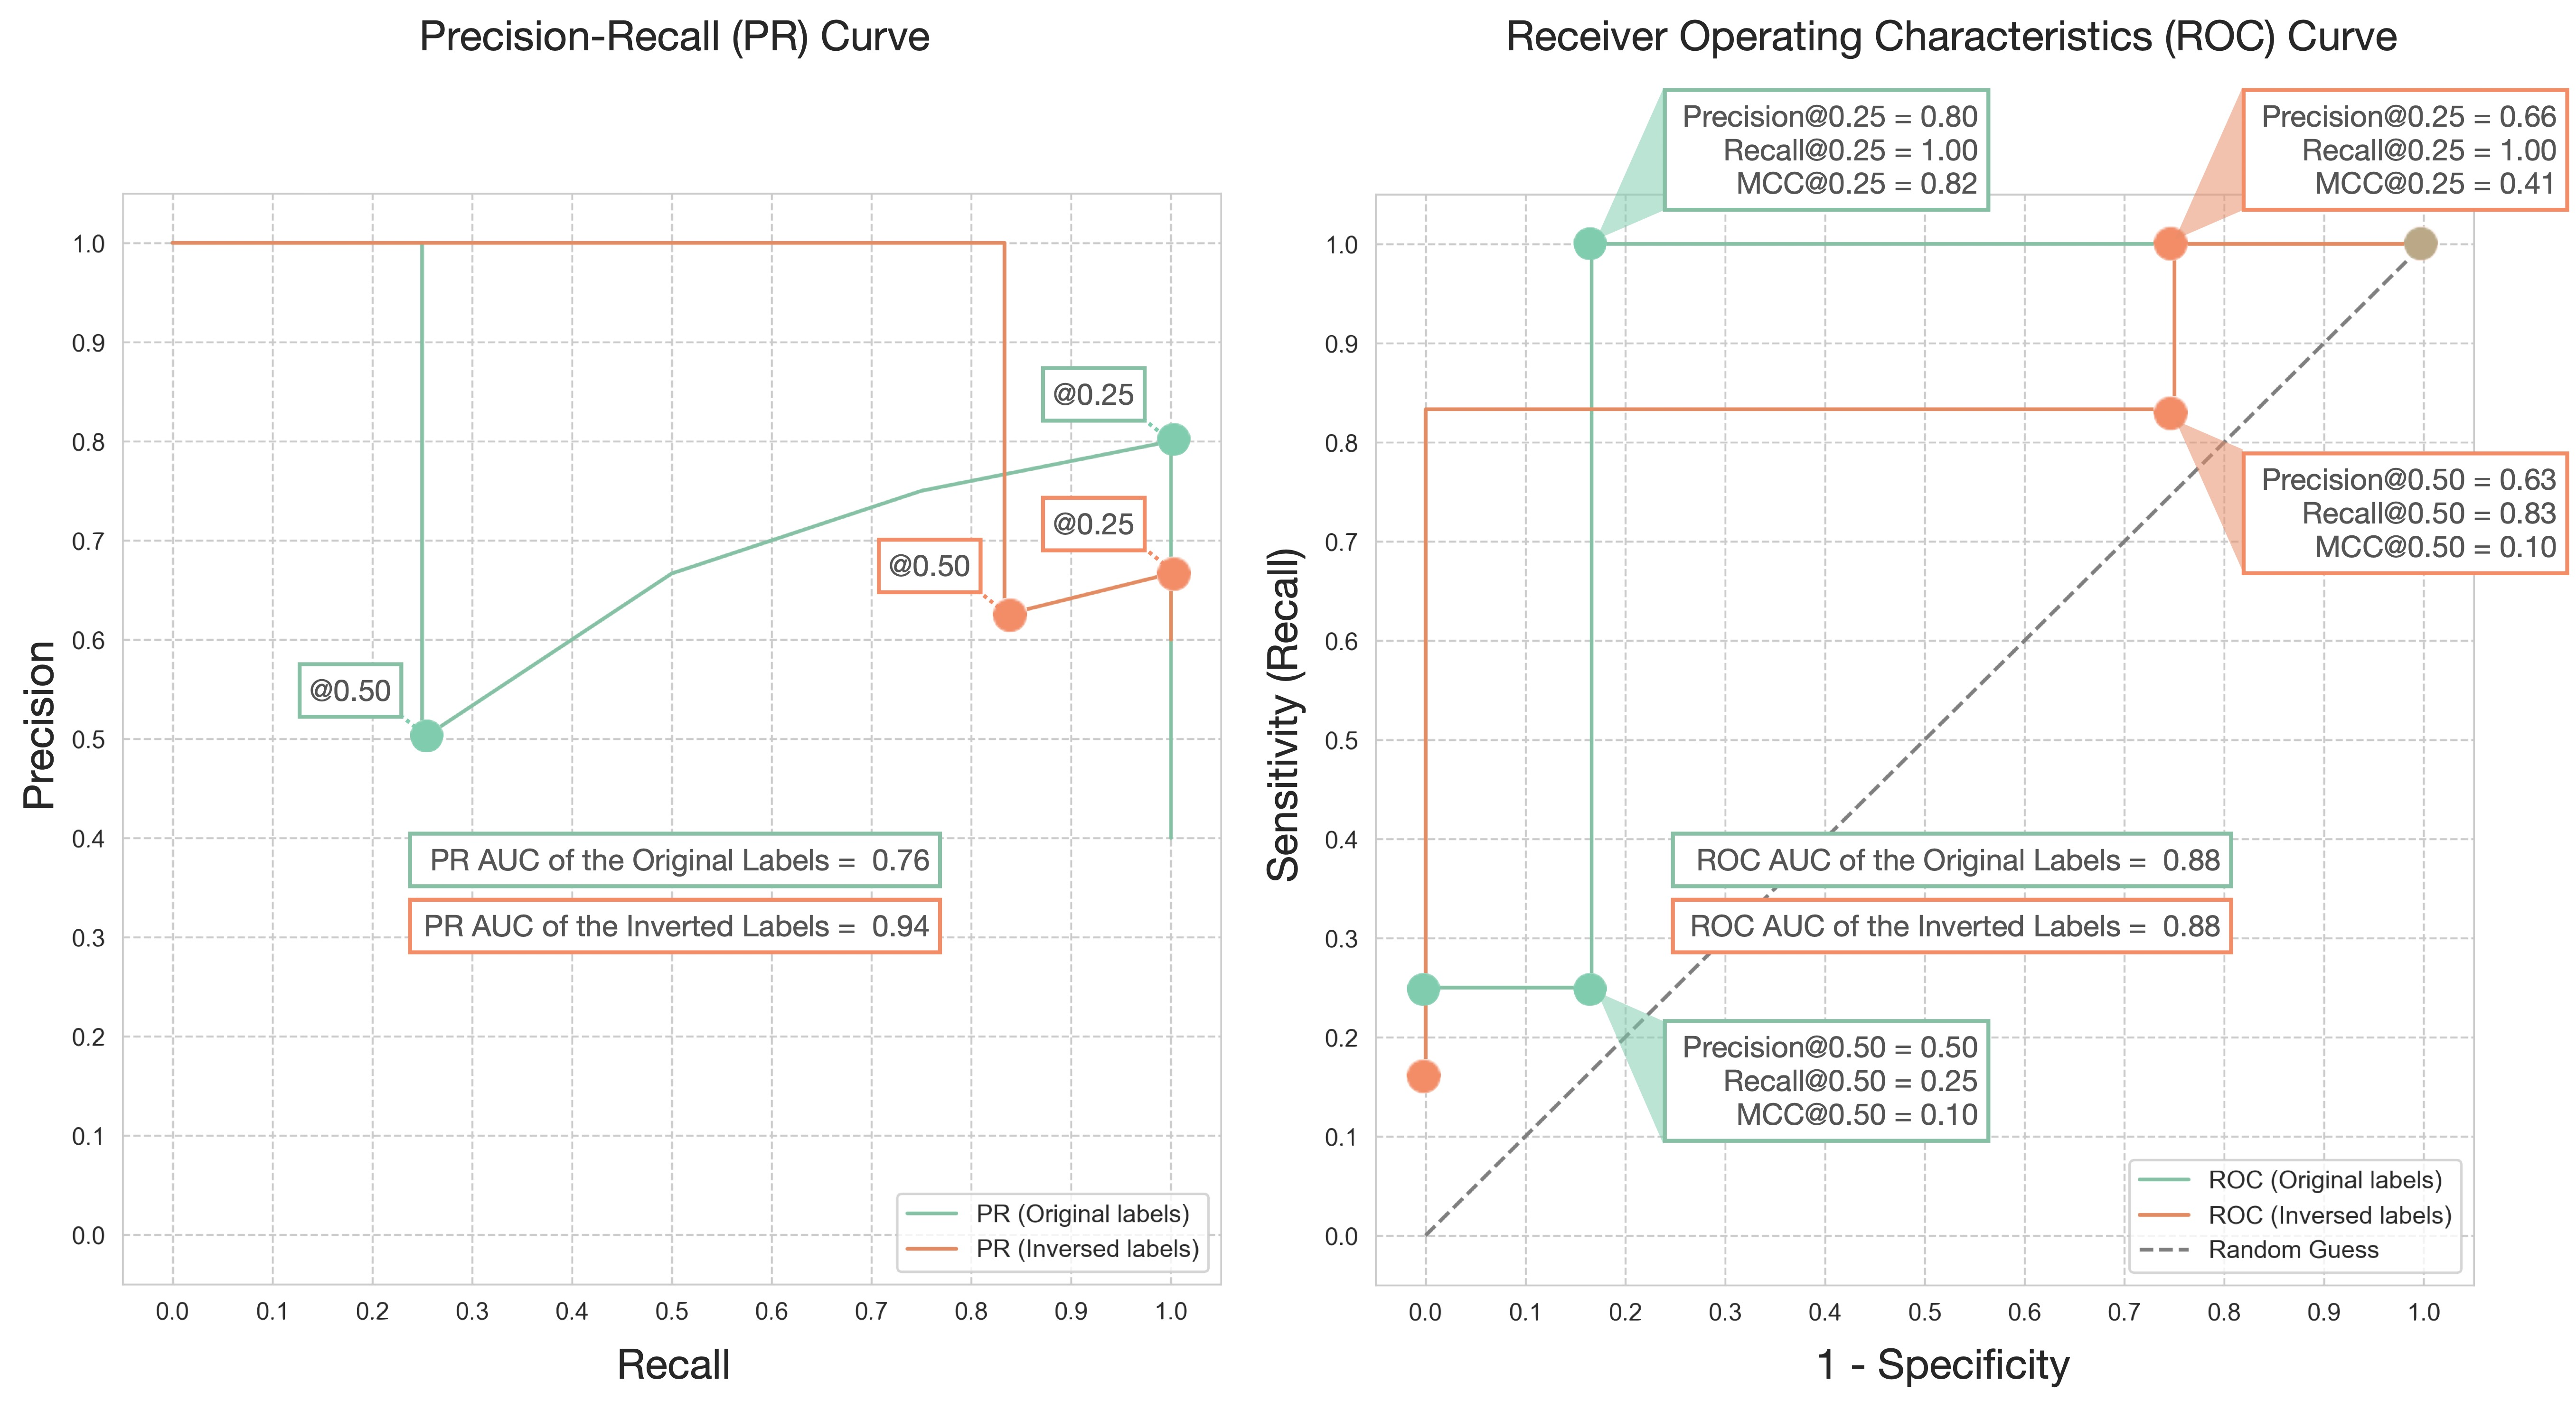
\includegraphics[width=1\textwidth]{fig_s5_curve.jpg}
    \caption{\textbf{(Left)} Precision-recall (PR) curve and \textbf{(Right)} Receiver operating characteristic (ROC) curve for the hypothetical example are displayed. The performance at confidence thresholds of 0.25 and 0.50 is highlighted. Original labels are marked in green, while inverted labels appear in orange. The Area Under the Curve (AUC) is depicted at the center of each curve.}
    \label{fig:s5_curve}
\end{figure}

However, it is worth re-emphasizing that precision and recall focus predominantly on positive samples. Inappropriately assigning a predominant background event as the positive class can lead to skewed interpretations. This pitfall is demonstrated in this example by inverting the labels. At a threshold of 0.50, precision increases from 0.50 to 0.63, and recall jumps from 0.25 to 0.83. With the threshold set at 0.25, precision drops to 0.66 from 0.80, while recall remains unchanged. The PR AUC also rises from 0.76 to 0.94. Such shifts in metrics, driven merely by label rearrangement unrelated to the data or model characteristics, underscore the importance of label-invariant metrics that remain unaffected by label assignments.
Unlike metrics focusing solely on positive samples, the ROC curve accounts for both positive and negative samples, making it a label-invariant metric. Specificity is plotted on the x-axis and sensitivity on the y-axis, calculated at different thresholds (Figure ~\ref{fig:s5_curve}, Right). In this hypothetical example, the ROC curve demonstrates robustness and label-invariance with a consistent AUC of 0.875, regardless of whether the original or inverted labels are used.
Lastly, another label-invariant metric is MCC which provides a balanced assessment of both positive and negative samples. Considering MCC's balanced approach to evaluating model performance, this study introduces the concept of an MCC curve. This curve, which plots the MCC value against various threshold levels (Figure ~\ref{fig:s5_mcc}), serves as a powerful tool for identifying the optimal confidence thresholds for model predictions. By examining this curve, one can determine the specific threshold at which the MCC value peaks, thereby optimizing the model's performance. For example, when applied to the hypothetical example, the optimum MCC value of 0.82 was attained at a threshold of 0.25. This particular threshold corresponded to accuracy, precision, and recall values of 0.90, 0.75, and 1.00, respectively. Notably, the MCC curve retains its symmetry even when labels are reversed, affirming its status as a label-invariant measure. In scenarios with inverted labels, the maximum MCC value observed was 0.83, achieved at a threshold of 0.75, leading to accuracy, precision, and recall values of 0.90, 1.00, and 0.83, respectively. Such findings underscore the MCC's ability to provide a balanced and comprehensive assessment of both positive and negative samples, thereby reinforcing its utility as a versatile and effective metric for thorough model evaluation.

In conclusion, binary classification models are often evaluated using metrics focusing on positive samples, such as precision and recall. It is generally advisable to designate the event of interest as the positive class. Otherwise, these metrics can be misleading when the more common but less significant background event is mistakenly marked as the positive class. To circumvent this potential bias, adopting label-invariant metrics is recommended. These metrics offer a more balanced and reliable assessment of model performance. Notable examples of such metrics include the ROC curve and the proposed MCC curve by this review, both of which are unaffected by the choice of positive and negative class labels and are thus robust for a thorough model evaluation.
\begin{figure}[h]
    \centering
    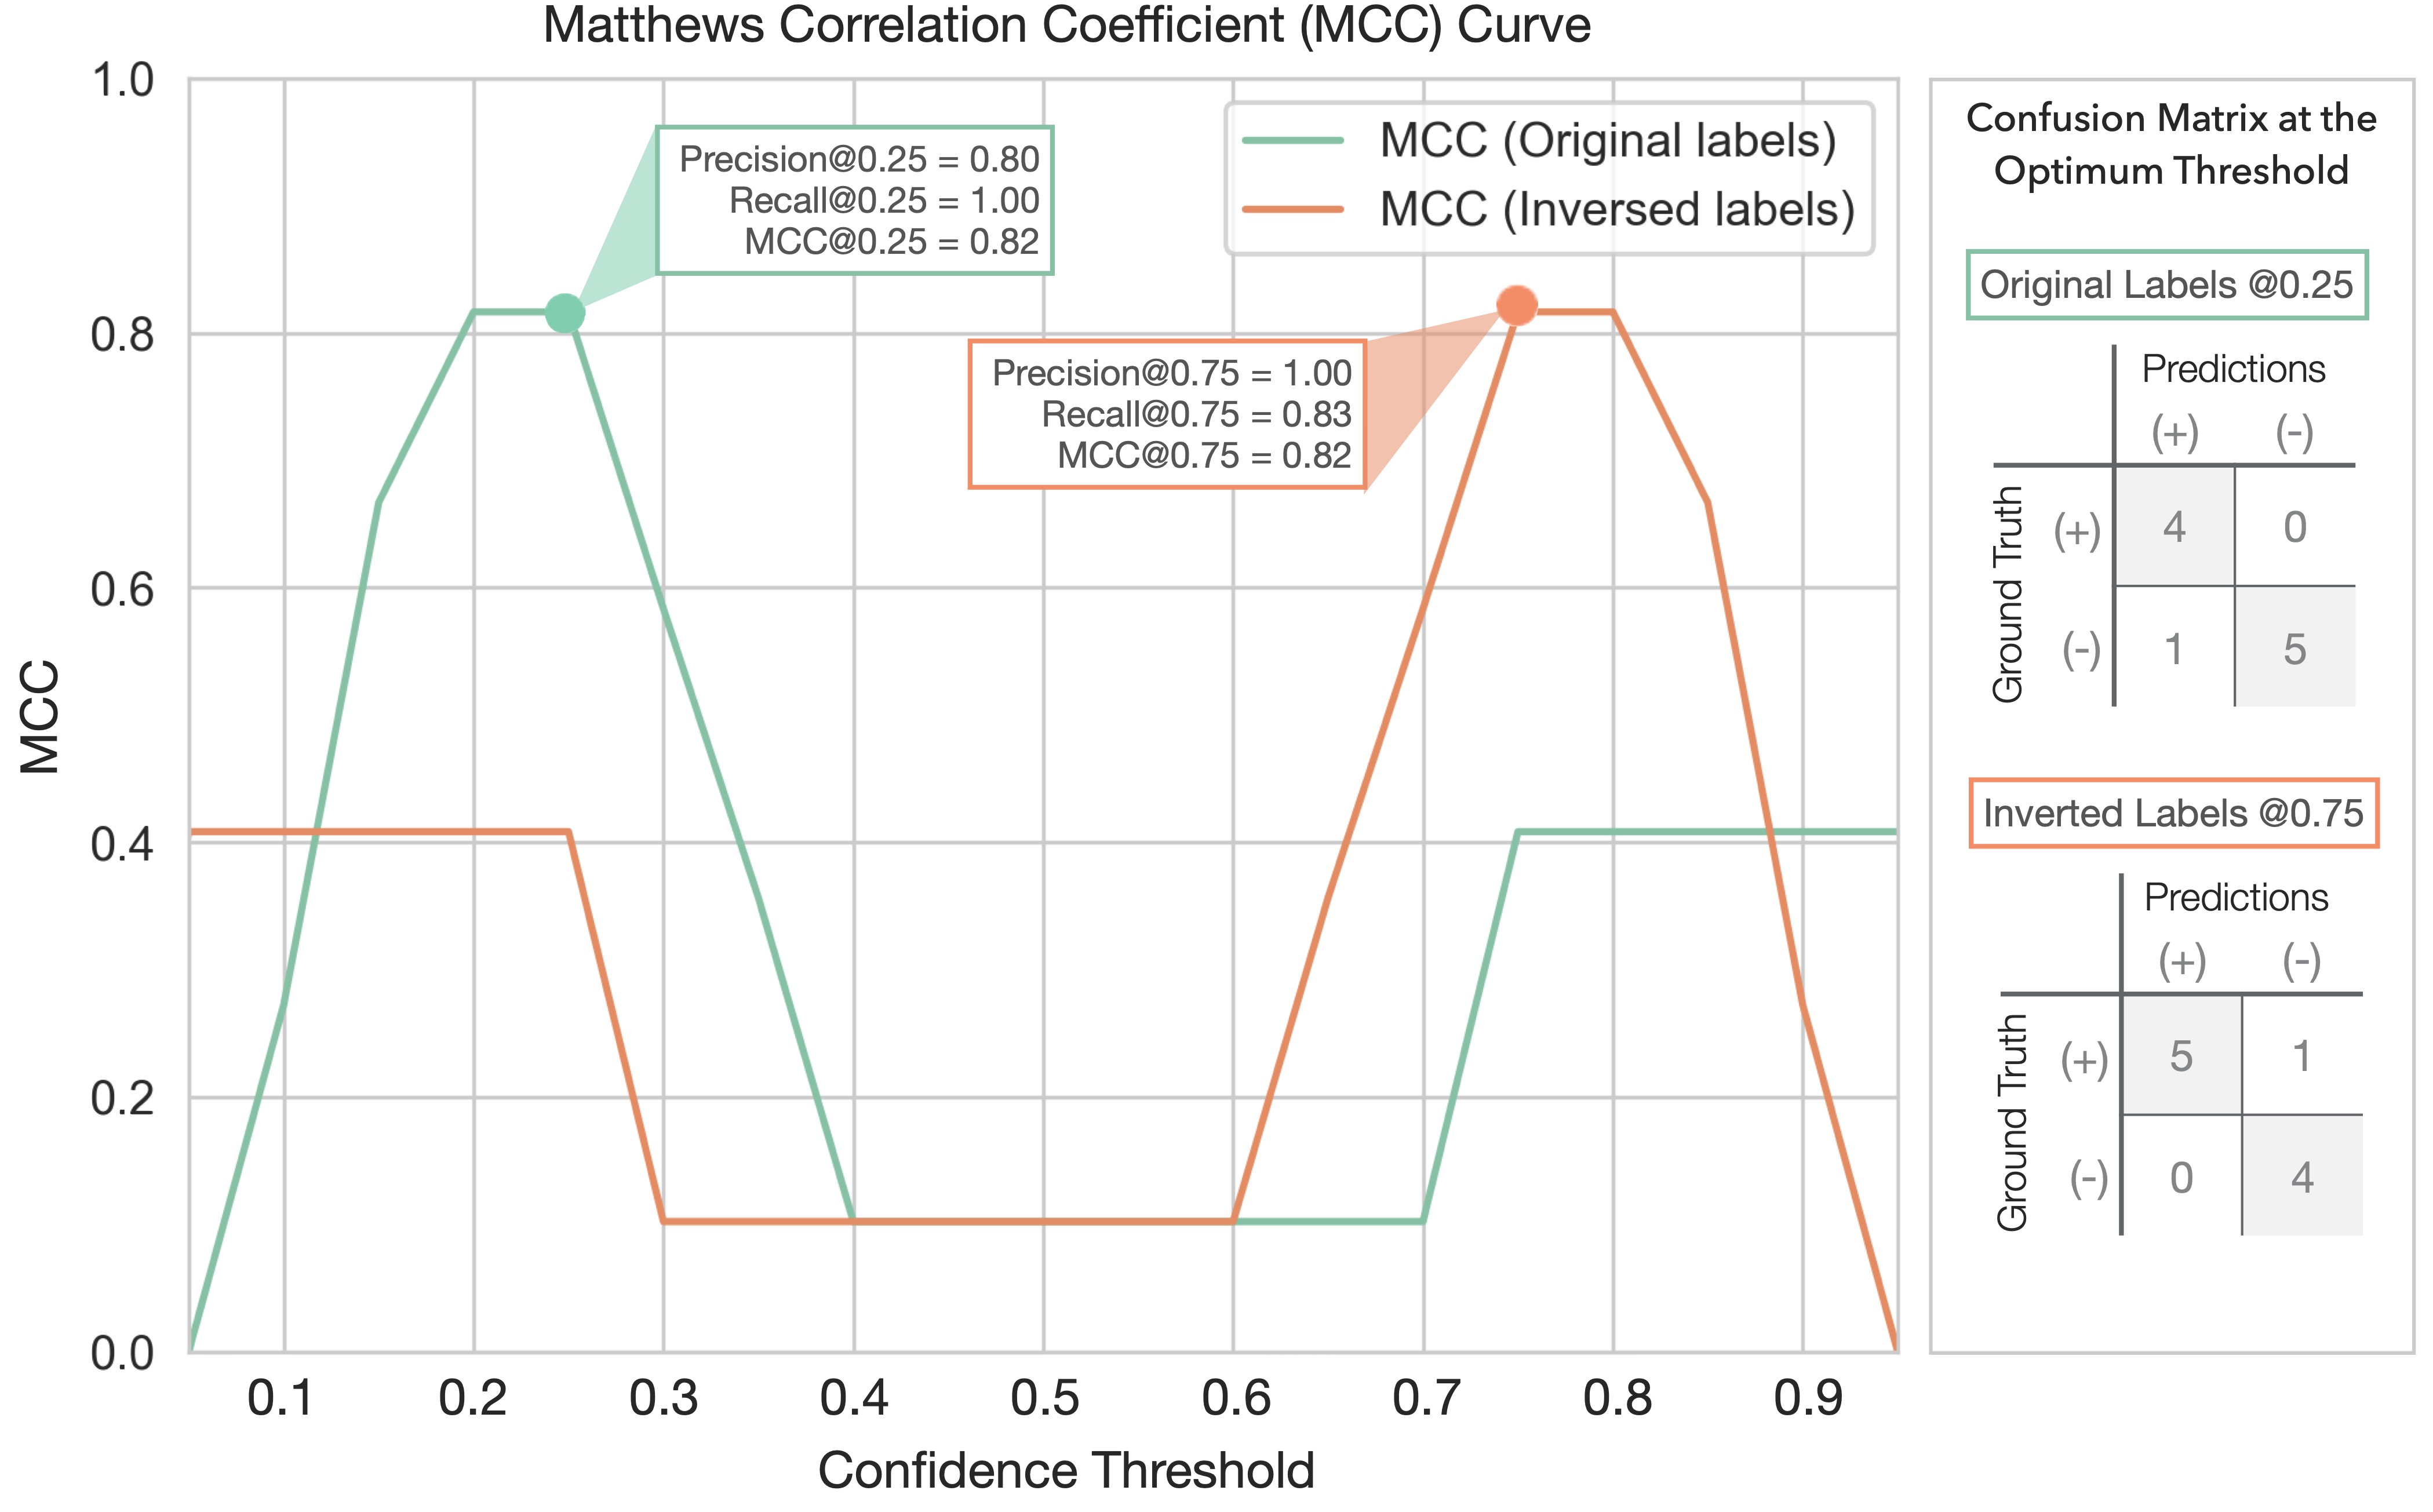
\includegraphics[width=.8\textwidth]{fig_s5_mcc.jpg}
    \caption{Matthews Correlation Coefficient (MCC) curve. A line chart plotting MCC at different thresholds for the hypothetical example. The optimal threshold is highlighted by the dot marks in green and orange for the original and inverted labels, respectively. The confusion matrix at the optimal threshold is displayed in the right panel.}
    \label{fig:s5_mcc}
\end{figure}
\input{content/_4_discussion.tex}


\section{Conclusion}
Your conclusion here

\section*{Acknowledgments}
This was was supported in part by......

%Bibliography
\bibliographystyle{unsrt}
\bibliography{references}

% just for references
\newpage
\section{Headings: first level}
\label{sec:headings}

\lipsum[4] See Section \ref{sec:headings}.

\subsection{Headings: second level}
\lipsum[5]
\begin{equation}
\xi _{ij}(t)=P(x_{t}=i,x_{t+1}=j|y,v,w;\theta)= {\frac {\alpha _{i}(t)a^{w_t}_{ij}\beta _{j}(t+1)b^{v_{t+1}}_{j}(y_{t+1})}{\sum _{i=1}^{N} \sum _{j=1}^{N} \alpha _{i}(t)a^{w_t}_{ij}\beta _{j}(t+1)b^{v_{t+1}}_{j}(y_{t+1})}}
\end{equation}

\subsubsection{Headings: third level}
\lipsum[6]

\paragraph{Paragraph}
\lipsum[7]

\section{Examples of citations, figures, tables, references}
\label{sec:others}
\lipsum[8] \cite{kour2014real,kour2014fast} and see \cite{hadash2018estimate}.

The documentation for \verb+natbib+ may be found at
\begin{center}
  \url{http://mirrors.ctan.org/macros/latex/contrib/natbib/natnotes.pdf}
\end{center}
Of note is the command \verb+\citet+, which produces citations
appropriate for use in inline text.  For example,
\begin{verbatim}
   \citet{hasselmo} investigated\dots
\end{verbatim}
produces
\begin{quote}
  Hasselmo, et al.\ (1995) investigated\dots
\end{quote}

\begin{center}
  \url{https://www.ctan.org/pkg/booktabs}
\end{center}

\subsection{Figures}
\lipsum[10] 
See Figure \ref{fig:fig1}. Here is how you add footnotes. \footnote{Sample of the first footnote.}
\lipsum[11] 

\begin{figure}
  \centering
  \fbox{\rule[-.5cm]{4cm}{4cm} \rule[-.5cm]{4cm}{0cm}}
  \caption{Sample figure caption.}
  \label{fig:fig1}
\end{figure}

\subsection{Tables}
\lipsum[12]
See awesome Table~\ref{tab:table}.

\begin{table}
 \caption{Sample table title}
  \centering
  \begin{tabular}{lll}
    \toprule
    \multicolumn{2}{c}{Part}                   \\
    \cmidrule(r){1-2}
    Name     & Description     & Size ($\mu$m) \\
    \midrule
    Dendrite & Input terminal  & $\sim$100     \\
    Axon     & Output terminal & $\sim$10      \\
    Soma     & Cell body       & up to $10^6$  \\
    \bottomrule
  \end{tabular}
  \label{tab:table}
\end{table}

\subsection{Lists}
\begin{itemize}
\item Lorem ipsum dolor sit amet
\item consectetur adipiscing elit. 
\item Aliquam dignissim blandit est, in dictum tortor gravida eget. In ac rutrum magna.
\end{itemize}


\end{document}
